%--------------------------------------------------------------------------------------------------%
%   Version:    1.0
%   Last Mod:   20190328    
%         By:   Gael Touquet gael.touquet@gmail.com
%   Author:     Juan Medina gael.touquet@gmail.com
%--------------------------------------------------------------------------------------------------%

%-------------------------------------------- PREAMBLE --------------------------------------------%
\documentclass[12pt,twoside]{report}
\usepackage[a4paper,width=150mm,headheight=110pt,top=25mm,bottom=25mm]{geometry}
\usepackage[utf8]{inputenc}
\usepackage{listings}
\usepackage{graphicx}
\usepackage{pgffor} 
\usepackage{float}
\usepackage{graphics} 
\usepackage{fancyhdr}
\usepackage{ptdr-definitions}

\graphicspath{{Images/}}

\usepackage[round, numbers,authoryear]{natbib}
\usepackage{color}
\usepackage[dvipsnames]{xcolor}

\definecolor{mycolor}{RGB}{30,75,180}
\definecolor{mycolor2}{RGB}{40,75,90}
% Lund colors
\definecolor{LUGreen}{RGB}{173,202,184}
\definecolor{LUPink}{RGB}{233,196,199}
\definecolor{LUBlue}{RGB}{0,0,128}
\definecolor{LUBronze}{RGB}{156,97,20}
\definecolor{LUblue}{RGB}{185,211,220}
\definecolor{LUGrey}{RGB}{77,76,68}

\usepackage[colorlinks = true,
            linkcolor = mycolor,
            urlcolor  = mycolor,
            citecolor = mycolor,
            anchorcolor = mycolor]{hyperref}

\usepackage[hypcap=true,font={small,it}]{caption}

\captionsetup{belowskip=2pt,aboveskip=2pt}
\bibliographystyle{abbrvnat}

\renewcommand{\chaptername}{}

\renewcommand{\figureautorefname}{figure} % lower case default ref
\renewcommand{\tableautorefname}{table} % lower case default ref
\newcommand{\latex}{\LaTeX\xspace}
\newcommand{\mcite}[1]{\textcolor{mycolor}{\citeauthor{#1} (\citeyear{#1})}}
\newcommand{\hcite}[1]{(\textcolor{mycolor}{\citeauthor{#1}, \citeyear{#1}})}
\newcommand{\colin}[1]{\textcolor{blue}{#1}}

%----------------------------------------------------------------------------------------------------%

%--------------------------------------------- DOCUMENT ---------------------------------------------%
\begin{document}
%\fancyhead[RO,LE]{}

% Title page
    \begin{titlepage}

\begin{center}

\includegraphics[scale= 0.5]{Images/Planche_UdL_LogoLyon1Sig_CoulRvb72dpi.jpg}
\end{center}

N\degree d'ordre NNT : xxx \\
\begin{center}
{\Large \textbf{THESE de DOCTORAT DE L'UNIVERSITE DE LYON}\\ }
operée au sein de \\ 
{ \textbf{L'Université Claude Bernard Lyon 1 }\\ }

\vspace{2em}
{ \textbf{Ecole Doctorale  } N° 52\\ }
{ \textbf{Ecole Doctorale de Physique et Astrophysique  } \\ }

\vspace{2em}
{ \textbf{Specialité du doctorat  } : Physique des particules\\ }
\vspace{4em}

 Soutenue publiquement le 25/10/2019 par : \\ 


\vspace{2em}

{\Large \textbf{Gael Touquet}}\\


\vspace{1em}

{\Large
\noindent\hfil\rule{0.7\textwidth}{1.5pt}\hfil\\
\vspace{.5em}
\textbf{Recherche d’un boson de Higgs supplémentaire du MSSM se désintégrant en deux leptons tau avec l’expérience CMS}\\
\noindent\hfil\rule{0.7\textwidth}{1.5pt}\hfil\\
}
\vspace{2em}



devant le jury compose de :

\vspace{1em}

{
\begin{tabular}{llllll}
Mme.   & Collard & Caroline  &  Directrice de recherche & CNRS      & Rapporteure \\
M.  & Lafaye & Rémi &  Directeur de recherche & CNRS   & Rapporteur\\
Mme.  & Petit  & Elisabeth &   Chargee de recherche & CNRS & Examinatrice\\
M.   & Tsimpis   & Dimitrios &  Professeur des universités & UCBL   & Examinateur \\
\\
M.   & Bernet  & Colin & Charge de recherche &UCBL   & Directeur de these
\end{tabular}
}
\end{center}

\vspace{1em}
\vfil



\end{titlepage}

% \begin{titlepage}
% 
\includegraphics{Images/LundLogoSEM.png}\\
% \vspace{2cm}
% Master's Programme in [xxx]
%     \begin{center}
%         \vspace*{1cm}
        
%         {\LARGE \textbf{[Title]}}
        
%         \vspace{0.5cm}
%         [Subtitle]
        
%         \vspace{1.5cm}
%         by \\
%         \vspace{1.5cm}
%       $[$Author's full name and \url{email address}$]$
                
%         \vspace{1.0cm}
%     \end{center}

% \noindent{
% \textcolor{red}{{\bf Abstract} (The Abstract is a short summary of what your thesis is about. It accurately reflects the content of the thesis providing information about the research problem, research aims, methods and procedures, results and implications. It is a short section. Abstracts give readers the opportunity to quickly see the main contents of the paper and enable them to decide whether the paper is of particular interest to their needs. This section will be one of the last sections that you write. No subheadings are used in an abstract.)
% }
% }
% \vfill
% \textcolor[rgb]{0.5,0.5,0.5}{
%     \begin{flushleft}
%     { \small
%     EKHM51 \\
%     Master’s Thesis (15 credits ECTS) \\
%     (Month) (Year) \\
%     Supervisor: [Full name] \\
%     Examiner: [Full name] \\
%     Word Count: \\
%     }
%     \end{flushleft}
% }
      
% \end{titlepage}

% Optional Chapters

    %\chapter*{Dedication}
    %\chapter*{Declaration}
    \chapter*{Acknowledgements}
    \textcolor{red}{It is usual, but not compulsory, to thank those who have been of particular help to you in completing the thesis.}

% Table of contents, list of figures, and list of tables
    {\hypersetup{linkcolor=black}
        \tableofcontents
        \listoffigures
        \listoftables
    }
        {\hypersetup{linkcolor=mycolor}}
    
% Introduction
    \chapter{Introduction} 
    Physics is the branch of science that intends to study Nature at its most fundamental level. As the properties of any object in Nature derive from its constituents, the most fundamental understanding of our universe relies on understanding the basic constituents of matter and its interactions. The theoretical and experimental efforts of generations of scientists have allowed us to zoom into the structure of matter with more and more precision, and to find new fascinating structures at every level. We now understand that chemistry is driven by the properties of atoms, and that each atom is comprised of electrons and an atomic nucleus, which is in turn made up of protons and neutrons, that are themselves made of quarks and gluons. These objects are, for now, considered to be the fundamental constituents of matter.

Particle physics is the branch of physics that specialises in the description of these fundamental constituents and their interactions. At this level, quantum mechanics dictate the rules and properties of every object and interaction. In this framework, small distances correspond to large energy scales, so studying the smallest constituents of nature requires a theoretical understanding of high-energy processes and advanced technology to produce them in a laboratory. Thus the field of particle physics is also often called high-energy physics.

Indeed, to understand the properties and the laws governing the particles of Nature, any theory must be confronted with observations. Experiments have therefore been designed to test the properties of theories such as the standard model (SM) of particle physics, a unified quantum field theory which was formulated in the 1960s and early 1970s. This theory is one of the most rigorous and precise ever created, and it has passed innumerable experimental tests over the past decades. For instance, the SM predicted the existence of several elementary particles, such as the $\mathrm{W^{\pm}}$ and $\mathrm{Z}$ bosons, gluons and the top quark, before they were experimentally discovered.

The last missing piece of the SM pending experimental confirmation was the existence of a Higgs boson. In the SM, elementary particles gain their masses by interacting with a field known as the Higgs field, manifesting itself as Higgs bosons. The Englert-Brout-Higgs mechanism that makes this possible via a spontaneous breaking of electroweak symmetry was predicted by three independent groups in 1964.

To test for the existence of this last piece of the SM, the Large Hadron Collider (LHC) was built. There, massive elementary particles such as these potential Higgs bosons can be produced in energetic particle collisions, converting the energy of the colliding particles, which is mostly kinetic energy, into mass. In 2012, after a few years of collision data gathering, the ATLAS and CMS experiments at the LHC discovered a new particle with a mass of approximately $125\,\mathrm{GeV}$, which was later confirmed to be a Higgs boson. The discovery completed the era of experimental searches for new particles guided by the SM.

While the SM is one of the most successful theories developed this far, it suffers from
both experimental and theoretical shortcomings. These shortcomings suggest that the SM is not a complete description of nature, but rather a low-energy approximation of a more general theory. Many candidates for this beyond the Standard Model (BSM) theory have been proposed. The minimally supersymmetric extension of the standard model is one such BSM model that adds a new symmetry on top of the existing ones in the SM, leading to the prediction of extra particles. This model, as most of these BSM theories, predicts an extended Higgs sector, with a spectrum of Higgs bosons with different masses, charges, and other properties.  These models are constrained, but not excluded, by the measured properties of the $125\,\mathrm{GeV}$ boson. Two-Higgs-doublet models (2HDMs) predict five different Higgs bosons: two neutral CP-even particles h and H, one neutral CP-odd particle A, and two charged Higgs bosons $\mathrm{H^{\pm}}$. The observation of additional Higgs bosons would provide direct evidence for the existence of BSM physics, and could push the searches towards other predicted particles of the MSSM.

In this thesis, a theoretical context focusing on the SM and the MSSM is given in chapter \ref{sec:TheoryChapter}. Chapter \ref{sec:CMSchapter} provides the experimental context, namely the CMS experiment of the LHC. Chapter \ref{sec:RECNNchapter} details a new approach to hadronic tau identification, whose goal is to improve sensitivity in the search .for extra heavy neutral Higgs bosons, detailed in chapter \ref{sec:Analysis}. This search is performed, based on proton-proton collisions  provided  by  the  LHC  at  a  center-of-mass  energy  of $13\,\mathrm{TeV}$ and collected by the CMS experiment in 2017.  The amount of data corresponds to an integrated luminosity of $41.5\,fb^{-1}$.




% Particle physics describes the fundamental constituents of matter, and their interactions, through the Standard Model, a quantum field theory. This theory has proven itself successful by predicting all observations made from particle colliders since it was first described in the 1960s. Its most recent achievement is predicting the existence of the Higgs boson, discovered for the first time in 2012.

% But the Standard Model has not successfully described all observations from nature. Many of those observation leads to considering the Standard Model as an effective theory of a more fundamental model.  First, gravitation is not included in the fundamental interactions. Then the discovery of neutrino oscillation, and therefore the massive nature of neutrinos, was not predicted. Dark matter and dark energy, estimated to represent $95\,\%$ of the energy content of the universe, is not explained either. Those lacks have inspired many theories beyond the Standard Model. Since the standard model relied heavily on symmetries, many of the new theories have postulated the existence of a previously unknown symmetry. One of such theory is super-symmetry, relying on the existence of a boson-fermion symmetry. When developed, this new theory predicts the existence of additionnal neutral Higgs bosons that can all potentially decay to a pair of tau leptons.

% The LHC was built in order to experimentally test the validity of the Standard Model, measure its parameters, and even search for evidence of other physics. This powerful collider was built to reach energy scales never explored before in collider experiments. Two of the four major experiments built around the collision points of the LHC have both the goal of measuring the Standard Model parameters and  search for evidence of physics beyond the standard Model. Those experiments were already successful in discovering the Standard Model Higgs boson in 2012.

% The work presented in this thesis was done as part of the CMS collaboration. The first chapter details the theoretical context, introducing the Standard model and the Minimally Supersymmetric extension of the Standard Model. The second chapter describes the CMS experiment, which provides the experimental context. The third chapter details the standard hadronic tau decay identification technique as well as a new neural network based approach. Finally, the fourth chapter describes the search for a neutral heavy Higgs boson decaying to a pair of hadronically decaying taus.
     
% The CMS experiment
    \chapter{The CMS experiment}
    Chapeau :

\section{The Large Hadron Collider}


\section{CMS detector overview}

\subsection{Tracker}

\subsection{Electromagnetic calorimeter}

\subsection{Hadronic calorimeter}

\subsection{Muon chambers}

\subsection{Trigger system}

LHC rate too big for bandwidth capabilities => trigger system to only save relevant event

L1 - HLT trigger (final point = need reconstruction system if we want to have physics-based triggering)

\section{Event reconstruction}

\subsection{Particle flow}

tracks, clusters, linking

charged hadrons, photons, neutral hadrons, electrons, muons

\subsection{Jets}

what is a jet

JEC (before resudial)

\subsection{Missing transverse momentum (MET)}

\subsection{Hadronic $\tau$ ( $\tau_{h}$ )}

basic tau identification, mention seeding jets, refer to next chapter

\section{Simulation}

\subsection{Hard process} 

Generator(s)

\subsection{Detectors and interactions}

detector simulation, interactions

reconstruction

\subsection{Corrections}

\begin{enumerate}
\item JEC residual
\item pile up
\item ...
\end{enumerate}
    
% A recursive neural network for \tau_{h} identification
    \chapter{A recursive neural network for $\tau_{h}$ identification}
    
As seen before in sec \ref{sec:tau_lepton}, when a $\tau$ is produced in a collision, it can decay into several different final states.
Hadronic final states, denoted \tauh, represent about 65\% of tau decays.
These hadronic final states are characterised by one or three charged hadrons with or without \pizero . But similar particles can be reconstructed from other processes and decays, such as events involving QCD jets.
Since these QCD jets greatly outnumber \tauh in the final states of proton-proton collisions at the LHC, \tauh identification algorithms have been designed in CMS to reject QCD jets as much as possible while keeping a \tauh identification efficiency somewhere between 35\% and 70\%, depending on the purity needed by the analyses. Identification is performed on a jet basis, meaning algorithms classify all reconstructed jets as either background, meaning QCD jets, or signal, meaning \tauh decay products.
The standard \tauh identification algorithm used in CMS, which will be detailed in section \ref{sec:std_tau_id}, have reached excellent performance thanks to the use of particle-flow reconstruction but do not use its full potential. 

Deep learning algorithms have shown an ability to use available information as efficiently as possible for the task they are trained for. In the field of particle physics, for example, their use in heavy flavour jet-tagging \cite{btagging_NN} has shown significant improvements over previously used techniques. These networks show best results when their design, or architecture, simplifies the task at hand. New architectures specifically intended for high energy proton-proton collisions have shown promising results. One such architecture is the Recursive Neural Network (RecNN) \cite{Louppe:2017ipp} used to identify boosted jets originating from hadronically decaying W bosons. Deep learning techniques will be introduced by level of complexity leading to the RecNN in section \ref{sec:NN}. This architecture has been adapted to \tauh identification, as it is a similar task. The adaptations of this architecture as well as some improvements that have been implemented will be presented in section \ref{sec:RecNN}, along with the reached performance.

\section{The standard CMS hadronic $\tau$ decays identification}
\label{sec:std_tau_id}
\subsection{Decay mode finding}

First, the particles of the reconstructed jet are fed as input to the hadrons-plus-strip (HPS) algorithm \cite{tauh_reconstruction} to reconstruct and identify \tauh candidates. A first selection is the requirement that reconstructed jets have $\pt > 14\,\mathrm{GeV}$ and $|\eta| < 2.5$.
The constituent particles are combined into \tauh candidates compatible with one of the main $\tau$ decay modes, $\tau^- \rightarrow h^- \nu_\tau$, $\tau^- \rightarrow h^- \pizero \nu_\tau$, $\tau^- \rightarrow h^- \pizero \pizero \nu_\tau$, $\tau^- \rightarrow h^- h^+ h^- \nu_\tau$, and charge conjugates. The decay mode $\tau^- \rightarrow h^- h^+ h^- \pizero \nu_\tau$ is not considered owing to its relatively small branching fraction and high contamination from quark and gluon jets.

The \pizero produced in some decay modes have a mean life of about $9 \times 10^{-17}\,\mathrm{s}$ and about $99\%$ of their decays lead to two photons. Because of the large amount of material in the tracker, illustrated in figure \ref{fig:tracker_material}, photons often convert before reaching the ECAL. The resulting electrons and positrons can be identified as such by the PF algorithm or, in the case their track is not reconstructed, as photons displaced along the $\phi$ direction because their trajectory is bent by the magnetic field.
These neutral pions are therefore obtained by adding iteratively reconstructed photons and electrons located in a strip of size $0.05 \times 0.20$ in the ($\eta$,$\phi$) plane:
\begin{itemize}
    \item Every reconstructed electrons and photons of $\pt > 0.5\,\mathrm{GeV}$ in the strip are added iteratively from highest to lowest \pt.
    \item At every step, the position of the center of the strip is re-computed as a \pt-weighted average of the position of all constituents.
    \item Any electron or photon not included in an existing strip is used as seed to another new strip.
\end{itemize}

\tauh candidates are then formed by creating all combinations of either one or three charged-particle and up to two strips in the jet.
Each \tauh candidate is then required to have a mass compatible with its decay mode and to have unit charge.
Collimation of the products are ensured by requiring all charged hadrons and neutral pions to be within a circle of radius $\Delta R = (2.8\,\mathrm{GeV})/\pt$ in the ($\eta$,$\phi$), which is called the signal cone.
The size of the signal cone is, however, not allowed to increase above 0.1 at low \pt, nor to decrease below 0.05 at high \pt. It decreases with \pt to account for the boost of the $\tau$ decay products. Finally, the highest \pt selected \tauh candidate in a given jet is retained. The four-momentum of the \tauh candidate is determined by summing the four-momenta of its constituent particles.

\subsection{Isolation}


\tauh candidates reconstructed from QCD jets are likely to be surrounded by other particles coming from the jet.
Isolation is therefore a powerful way to reject background QCD jets.

Two approaches are available : cut-based and multi-variate.

\paragraph{Cut-based} Isolation is computed from the \pt sum of charged particles and photons with $\pt > 0.5$ GeV within an isolation cone of $dR=0.5$ centered around the \tauh direction, excluding particles used to form the \tauh candidate. In order to mitigate pileup contribution, tracks associated to the considered charged particles are required to be compatible with the \tauh production vertex within a distance $\Delta z < 0.2\,\mathrm{cm}$ and $\Delta r < 0.03\,\mathrm{cm}$. The contribution from pileup is estimated as $\Delta \beta$ calculated from the contribution of charged displaced particles and removed as
\begin{equation}
    I_{\tau} = \sum_{charged, \Delta z<0.2 cm} \pt + max \Big\{ 0, \sum_{\gamma} \pt - \Delta\beta \Big\} \msep
    \label{eq:isolation}
\end{equation}
\begin{equation}
    \Delta \beta = 0.46 \sum_{charged,\Delta z>0.2 cm} \pt \mend
\end{equation}
Working points are defined by the thresholds on the value taken by the isolation defined in equation \ref{eq:isolation}. Usual working points such as loose, medium, tight are thresholds are 2.0, 1.0 and $0.8\,\mathrm{GeV}$ respectively.

\paragraph{Multi-variate} This method is based on decision trees. These are machine learning techniques that rely on finding the best successive cuts on the available variables to separate signal and background in a training set. Boosting is a method of combining many weakly classifying trees into a strong classifier. A BDT is trained on an appropriate choice of isolation variables to give best separation between QCD jets and \tauh : 
    \begin{itemize}
        \item charged- and neutral-particle isolation sums defined as in eq \ref{eq:isolation}.
        \item The reconstructed decay mode.
        \item the transverse impact parameter $d_0$ of the leading tack of the \tauh candidate and its significance $d_0 / \sigma_{d_0}$
        \item the distance between the $\tau$ production and decay vertices, $|\Vec{r}_{SV} - \Vec{r}_{PV}|$, and its significance $|\Vec{r}_{SV} - \Vec{r}_{PV}|/\sigma_{|\Vec{r}_{SV} - \Vec{r}_{PV}|}$, along with a flag indicating whether a decay vertex has successfully been reconstructed for a given \tauh candidate. The positions of the vertices, $\Vec{r}_{SV}$ and $\Vec{r}_{PV}$, are reconstructed using the adaptive vertex-fitter algorithm \cite{Waltenberger_2007}.
        \item More details on the variables can be found in \cite{tauh_reconstruction}.
    \end{itemize}

\subsection{Anti-leptons discriminants}

Electrons and muons can easily be misidentified as \tauh, particularly in the $h^{\pm}$ decay mode. Electrons radiating a bremsstrahlung photon that subsequently converts may also get reconstructed in the $h^{\pm}\pizero$ decay mode. Therefore discriminants have been developed to separate such leptons decays from real \tauh decay products.

Electrons are rejected by a BDT using observables that quantify the distribution in energy depositions in the ECAL and HCAL, in combination with observables sensitive to the amount of bremsstrahlung emitted along the leading track. The BDT also uses observables sensitive to the overall particle multiplicity, to distinguish electromagnetic from hadronic showers.
All these variables are listed in \cite{tauh_reconstruction}.
    
Muons are rejected by requiring that no track segments are found in at least two muon stations within a cone of size $\Delta R = 0.3$ around the \tauh direction. \tauh candidates are also rejected when the sum of the energies in the ECAL and HCAL corresponds to less than 20\% of the momentum of their leading track.

\subsection{Simulation of QCD jets and hadronic $\tau$ decays}
\label{sec:NN_datasets}

In order to compare the both classification methods, their performance is expressed in terms of signal efficiency and background rejection. To quantify these, and to provide a training set for our deep learning algorithm, datasets of QCD jets and hadronic tau decays have been selected from the simulated CMS datasets that were introduced in \ref{sec:cms_physics_event_generation}. Instead of simulating isolated QCD jets and \tauh separately, entire collision events are used as they provide a realistic environment similar to the one in which the classifier will be used.

Selected processes leading to \tauh and QCD jets in the final state are detailed in table \ref{tab:NN_b_s_diff}. QCD jets are obtained from QCD multijet events in which true \tauh are extremely rare, while \tauh are taken from events with true taus in the final state (MSSM $H\rightarrow \tau\tau$, DY $Z\rightarrow \tau\tau$).


The proton-proton collision events are generated with PYTHIA 8 \cite{SJOSTRAND2008852}, and are then processed by the CMS GEANT4 simulation, as detailed in section \ref{sec:cms_physics_event_generation}. The generation-level information is kept and will be referred to as gen level. All the information coming out of the detector simulation is fed to the CMS reconstruction algorithms, where the particle flow algorithm provides the list of reconstructed stable particles. Higher-level objects such as jets, are reconstructed by combining these particles using the clustering algorithms introduced in \ref{sec:jet_clustering}.

As stated before, the identification of \tauh and QCD jets is performed jet by jet. A reconstructed jet is defined as signal if it is selected from the genuine tau samples, and as background if selected from the QCD multijet samples. To ensure purity, some extra cuts are applied, these cuts can be found in table \ref{tab:NN_b_s_diff}.

The matching between reconstructed jets and gen level \tauh is done by ensuring their respective directions are aligned, meaning that the distance separating their orientation in the ($\eta ,\phi$) plane is required to be $\Delta R < 0.1$.


\begin{table}[ht]
    \caption{Provenance and cuts applied to reconstructed jets defining signal and background.}
    \centering
    \begin{adjustbox}{max width=\textwidth}
    \begin{tabular}{c||c|c}
        & \tauh (signal) & QCD jets (background) \\
        \hline \hline
        \multirow{3}{*}{Hard processes} & SUSY ggH $\rightarrow\tau\tau$ & \multirow{3}{*}{\begin{minipage}{0.4\textwidth}QCD multijets samples ordered by \pt : 15-30, 30-50, 50-80, 80-120, 120-170, 170-300 \end{minipage}} \\
        \cline{2-2}
         & SUSY bbH to $\rightarrow\tau\tau$ & \\
        \cline{2-2}
         & DY to tautau & \\
        \hline
        phase-space cuts & \multicolumn{2}{c}{$20<\pt<100 \text{ and } |\eta|<0.8$}\\
        \hline
        specific extra cuts & matched with gen-level \tauh & any \\
        \hline
    \end{tabular}
    \end{adjustbox}
    \label{tab:NN_b_s_diff}
\end{table}

Parts of these sets are also going to be used in the training of the deep learning algorithm. But biases coming from the difference between signal and background distribution can cause mistraining. For example, if both background and signal samples had different \pt distribution, the network could wrongly assume that the \pt of a reconstructed jet is correlated to its nature as a \tauh or a QCD jet, which should be avoided. To prevent this bias, the signal and background jets are split by \pt bins, and the selection signal and background jets is done in each \pt bin.

\subsection{Performance}


\begin{figure}
    \centering
    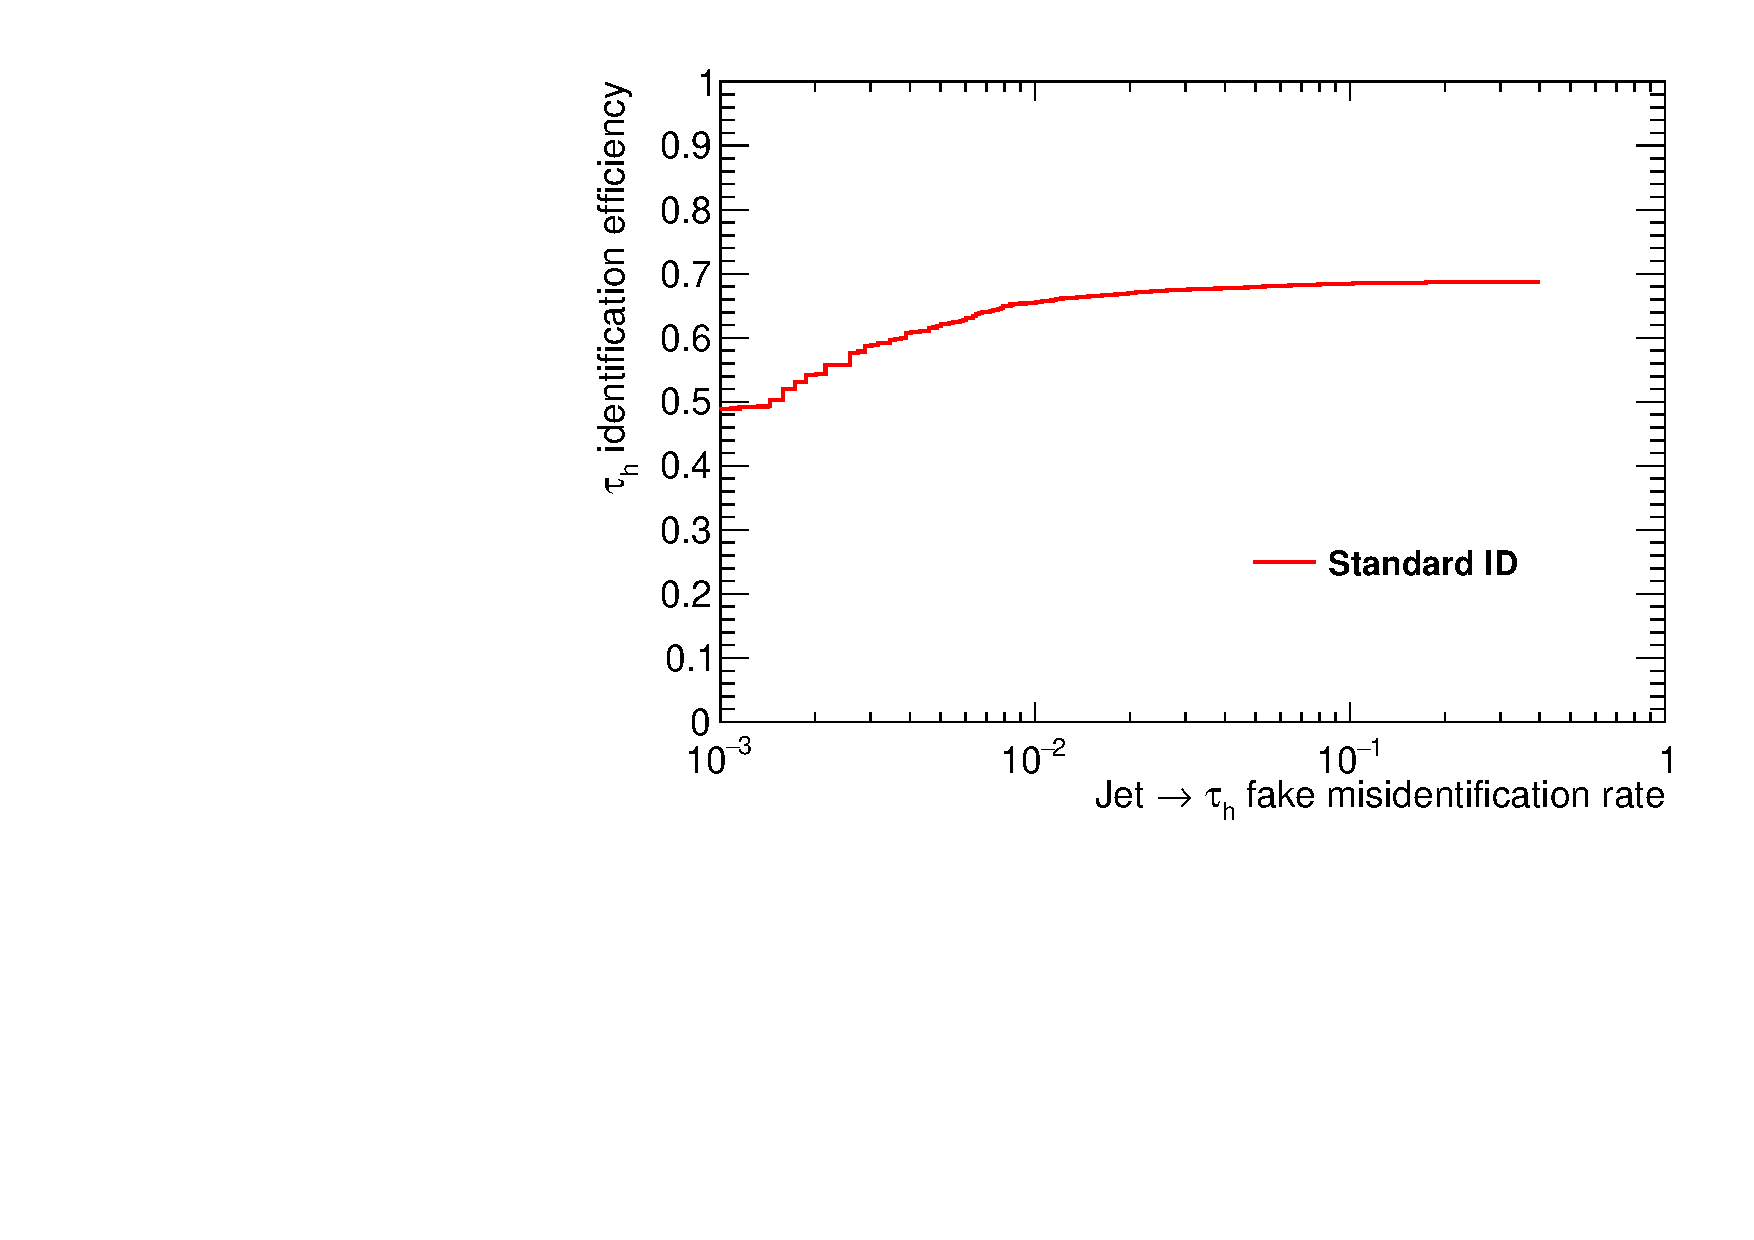
\includegraphics[width=\textwidth]{Images/ROC_comp_std.pdf}
    \caption{\tauh identification ROC curve for the standard method. The x axis is set to a logarithmic scale.}
    \label{fig:std_ROC}
\end{figure}

Performance is evaluated in terms of signal efficiency and background rejection. The signal efficiency is defined as the ratio of the number of well-tagged \tauh over the total number of \tauh in the selected population. The background rejection is similarly defined as the ratio of the number of well-tagged QCD jets over the total number of QCD jets in the population.

While the goal of a classifier is to tag objects as signal or background, most will instead provide with a score between 0 and 1. A score close to 0 is to be interpreted as very likely to be background, and a score close to 1 as very likely to be signal. This continuous score can then be translated into a discrete tag by the choice of a working point (WP) value. For a given WP, every reconstructed jet that scores below the WP value is then tagged as QCD jet, and every reconstructed jet that scores higher is tagged a \tauh. The values of the signal efficiency and background rejection can be measured for a continuous scan of WP values. The created curve in the signal efficiency vs background rejection space is called a Receiver Operating Characteristic (ROC) curve. The standard identification ROC curve is shown in figure \ref{fig:std_ROC}
A numerical figure of merit oftenly used to quantify the overall performance of a classifier is the area under the ROC curve, called ROC AUC, as it is maximum when signal efficiency and background rejection is perfect.
In our case, ROC AUC might not be the best figure of merit, as it doesn't take into account which regions are best covered by the technique. Indeed, in our case the standard identification technique is based on applying hard cuts such as decay mode finding and anti-lepton discriminant before scanning the score of the isolation BDT. This is why the ROC of the standard technique reaches a plateau, as the plateau corresponds to maximum efficiency allowed by the previous cuts.
QCD jets are also overwhelmingly more present in collisions than \tauh, meaning useful working points are in the region of high background rejection. 

\subsection{Intrinsic limitations}

The cut-based method relies on a single variable, namely isolation, to classify. The BDT-based method is an improvement on the cut-based method as it combines isolation with other variables susceptible to bring more information relevant to the classification process. But the BDT still takes a limited amount of information encoded into a strict number of variables. The construction of such variables do not take into account all the information gathered in the detection and reconstruction phases. A possible improvement should therefore be expected from using all the available information rather than a chosen subset. Deep learning techniques are conceptually adequate for such a task as they take all available information in and the process of such information is then completely derived from training.


\section{From a single neuron to recurrent networks}
\label{sec:NN}
Indeed, neural networks have brought a lot of new results in fields such as big data, image recognition and even pseudo-data generation.
Neural networks are based on processing units called neuron. These combination of such neurons into networks allows exponential possibilities of information processing. Those neural networks are then trained to give the desired output by a trial and error process on a set of examples. The set of examples given to a neural network is called a training set. By comparison with other trained techniques, the possibilities gained by the complexity of a neural network comes with a need for a bigger training set. The use of simulation simulation allows to have such a substantial training dataset.

The organisation of the neurons in the network is called architecture. Neural networks have shown their best achievements when their architectures are specifically designed for the task at hand.

\subsection{Basics : neurons, dense networks, deep learning}

\subsubsection{Neuron}

\begin{figure}
    \centering
    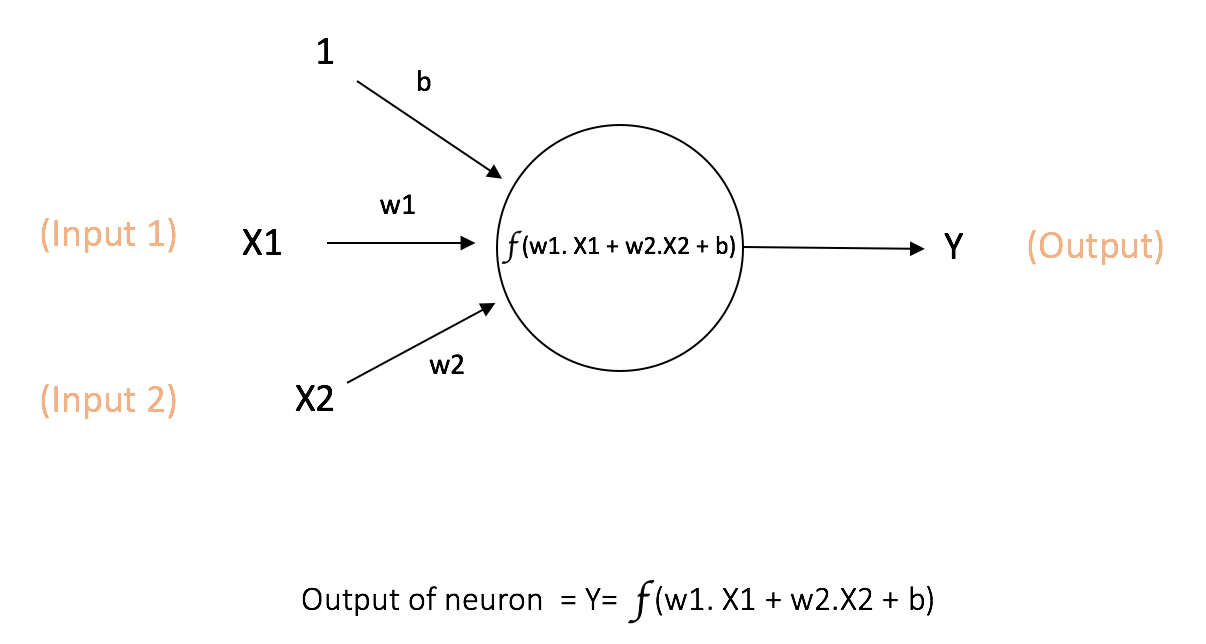
\includegraphics[width=0.8\textwidth]{Images/neuron_diagram}
    \caption{Diagram of a single neuron, in the case of two input variables.}
    \label{fig:neuron_diagram}
\end{figure}


\begin{figure}
    \centering
    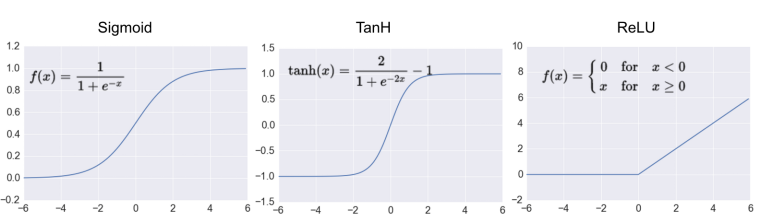
\includegraphics[width=\textwidth]{Images/activation_functions.png}
    \caption{Some activation functions and their visualisation.}
    \label{fig:activation_functions}
\end{figure}

A neuron is defined by an activation function $f$, a set of scalar weights $wi$ and a bias $b$. It takes a number of input variables denoted $X_i$ and produces as output the result of $f(\sum w_i\times X_i + b)$. The layout of a neuron taking two inputs is illustrated in figure \ref{fig:neuron_diagram}. The weighted input is also defined as $z = \sum w_i\times X_i + b$, and the output of the neuron becomes $f(z)$. The function is called activation function and is chosen among nonlinear differentiable functions. Some examples of widely used activation function are illustrated in figure \ref{fig:activation_functions}.

\subsubsection{Densely connected network}


\begin{figure}
    \centering
    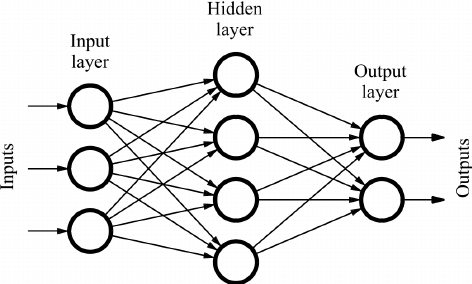
\includegraphics[width=0.5\textwidth]{Images/dense_network.png}
    \caption{Diagram of an example of a feed-forward densely connected network with 3 input variables, 4 neurons in the hidden layer and 2 output neurons.}
    \label{fig:dense_network}
\end{figure}

A network can be created from neurons by connecting their input and outputs. A simple case is the feed-forward densely connected network, such as shown in figure \ref{fig:dense_network}. In this architecture, neurons are organised by layers, with each neuron's output being one of the inputs of the neurons in the next layer. The first layer takes the variables of the task as inputs. Then the information is propagated through each neuron evaluation of its activation function. The output of the last layers is then considered the output of the network associated with the given set of inputs. An architecture is called feed forward when there is no cycle in the propagation of the evaluation from inputs to outputs. Such an architecture creates the possibility of approximating theoretically any task, as stated by the Universal approximation theorem states \cite{Cybenko1989}, as long as the activation function used in the neurons are non-linear.

\subsubsection{Training: loss function and backpropagation}

In order to find the set of weights and bias that allows the network to perform the desired task, the network is trained.
As previously mentionned, the training phase relies on a set of examples of inputs associated with their targeted output value. The training is done iteratively. The first step is comparing the output of the network for a set of inputs to the desired output. This comparison is quantified through the use of a metric called the loss function. The arguments of the loss function are the output of the network and the desired output. The loss function is required to be a differentiable function and is designed to reach a minimum when these arguments are equal, meaning the output of the network is the desired value. Training the network to perform the task is therefore equivalent to change the network parameters (weights and biases) to minimize the value of the loss function for the whole training set, provided the training set is a representative sample of the global population.

But the space of configurations of the weights and biases of the network has a huge dimensionnality. The iterative process of training the network case by case can then lead to stagnation if examples are evaluated and parameters adapted for each example of the training set. To avoid this stagnation, the parameters are changed to minimize the average of the loss function over a number of examples, called mini-batch. The number of examples in each mini-batch is referred to as the mini-batch size.

The way the parameters are changed to minimize the loss function depends on which optimizer algorithm is used. Most optimizers rely on backpropagation, meaning the variation that should undergo a parameter is computed by propagating the change of the loss function backwards through all the layers of neurons between the output of the network and the considered neuron using the chain rule.\newline


A classical problem that can occur in the training of neural networks is the existence of local minima of the loss function. Indeed, local minima can lead to a sub-optimal training, as it prevents the network from reaching a potentially lower global minimum. To mitigate such effects, diminishing learning rates as well as momentum-based optimizers are used. The learning rate is a simple scalar that multiplies the changes in parameters for a given change in loss. By starting at a high value of this learning rate, it is possible to avoid local minima that are too small. After several iterations of training, this rate can be lowered to help reach the lowest point of the minimum. 

Momentum-based optimizers try to avoid minimums by multiplying the learning rate by a factor proportional to the gain of the last step. Indeed, the more a training step helped minimizing the loss function, the bigger the next step, avoiding local minima on the way to a global minimum.\newline

Backpropagation comes with another important problem called vanishing gradients. This roughly is due to output of a neuron being generally relatively small compared to the input of a neuron. Indeed, an activation function such as the sigmoid, illustrated in figure \ref{fig:activation_functions}, can lead to states where the derivative is close to 0. But backpropagation relies on the derivatives of the cost function with respect to the parameters being derived using the chain rule backward from the last layer. This means the more layers are in between a neuron and the final layer, the more likely it is that its parameters will update based on the derivative that is close to 0. In other words, this means that a change in the parameters of a neuron in an early layer will have a relatively small effect on the loss compared to a similar change in the later layers. In the training, this leads to a slower training of the early layers compared than the last layers. Therefore, a very deep network, meaning many layers, will explore the sapce of its parameters very slowly compared to a shallow network. This can lead to much longer training stages, and even stagnation of the overall performance, meaning the network does not train. This is mitigated by the use of activation function such as the ReLU, which is defined as $f(x)=0$ for $x < 0$ and $f(x)=x$ for $x \geq 0$ as illustrated in figure \ref{fig:activation_functions}. This activation function avoids the small derivative by not requiring its output to be between 0 and 1. The use of cross-entropy as a loss function also allows to mitigate the vanishing gradients problem, as the derivative of the activation function cancels out in the computation of the derivative of the cost function with respect to a parameter of the network \cite{NN_book}. One can also mitigate further this problem by designing an architectural workaround, avoiding deep network when possible, for example using recurrent neural networks, which are introduced in the following section.



\subsection{Recurrent neural networks}

\begin{figure}
    \centering
    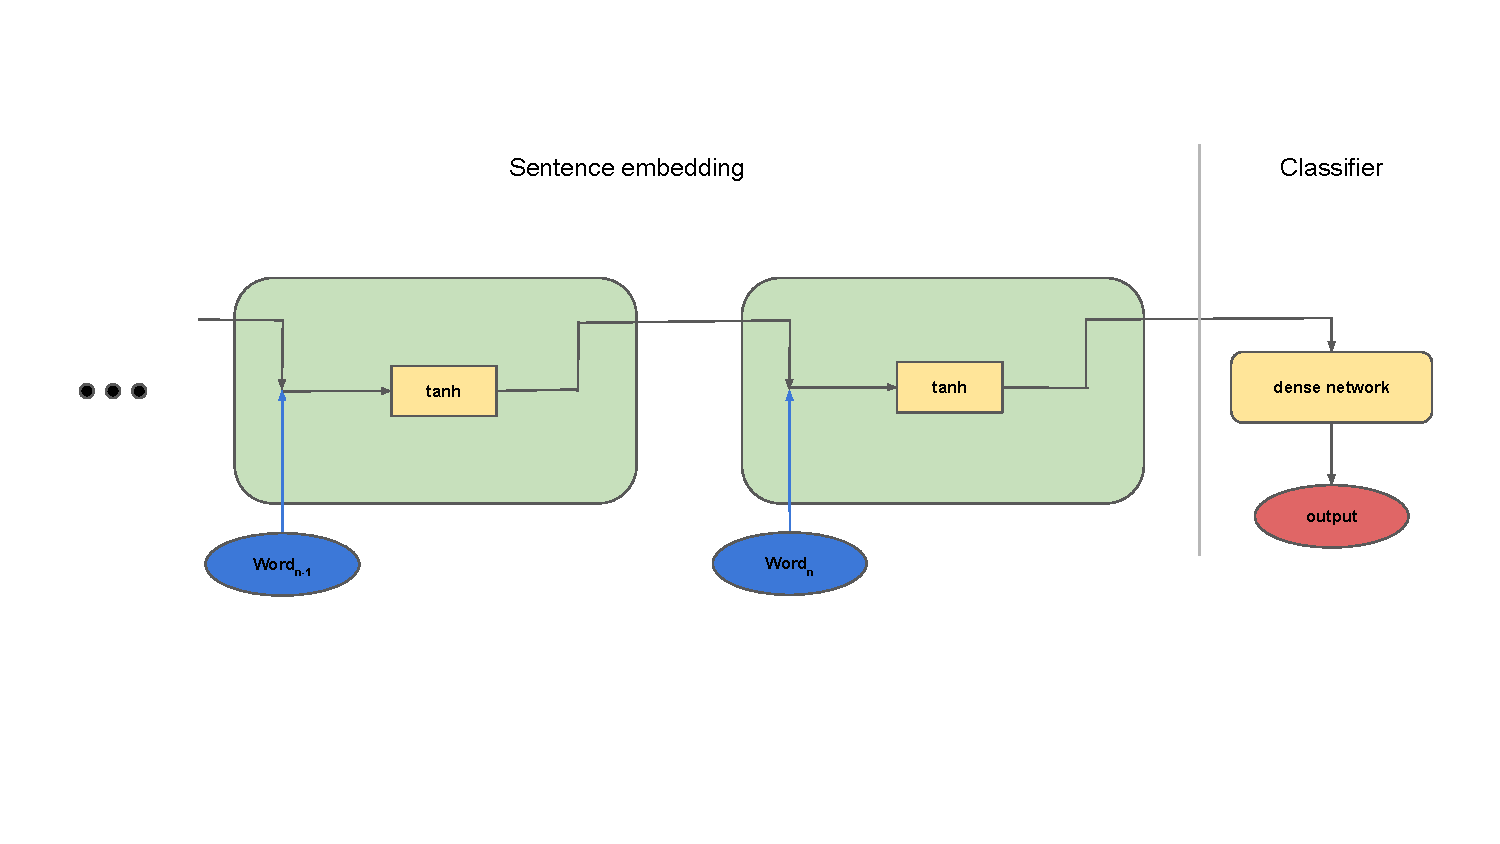
\includegraphics[width=\textwidth]{Images/Schema_RNN.pdf}
    \caption{Diagram of the iterative evaluation of a recurrent neural network in the language processing case. Only the two last iteration corresponding to the two last word of a sentence is represented. The green boxes represent several iteration of the same unit. The yellow rectangular boxes represent a single neuron layer and the rounded yellow box represent a dense network, which can made of several layers.}
    \label{fig:recurrent_network}
\end{figure}

The dense neural network that has been introduced has a limiting characteristic that limits its usage in our case. In order to use all the information available in jets, all the characteristics of the particles of each jet must be fed into the network. But each jet has a different number of particle, and a dense network cannot accommodate its number of input on a case-by-case basis. A category of architectures, which are designed to accommodate such a varying number of inputs, exist and those architectures are referred to as recurrent neural networks (RNNs). Those networks have been particularly useful in language processing tasks. Indeed, language processing have a similar varying number of inputs requirements, as the number of words changes in different sentences. RNNs are going to be introduced here in the case of an example task of classifying sentences as positive or negative.

Every RNN is separable into two distinct part. A first part has the goal of embedding the information gathered from the inputs into a fixed-size array of values. The second part is a dense neural network that takes the elements of this array as its inputs, and its output is considered the output of the RNN as a whole. The embedding part consists in applying a unit iteratively on each input element, in this case each word. The output of the previous iteration is also taken as a secondary input. The composition of a unit in terms of network layers and information flow then defines a specific RNN architecture. A simple case of RNN architecture is illustrated in Figure \ref{fig:recurrent_network}.

While this architecture has the advantage of being able to accomodate inputs of varying size, it also benefits from the fact that the same embedding unit is applied at each iteration, with the same parameters. This mitigates the vanishing gradient problem, as all parameters of the network are evaluated close to the final layer. Conceptually, this allows the use of a small amount of layers by taking advantage of the symmetries of the inputs. 

\subsection{Recursive neural networks}
\label{sec:RecNN}


\begin{figure}
    \centering
    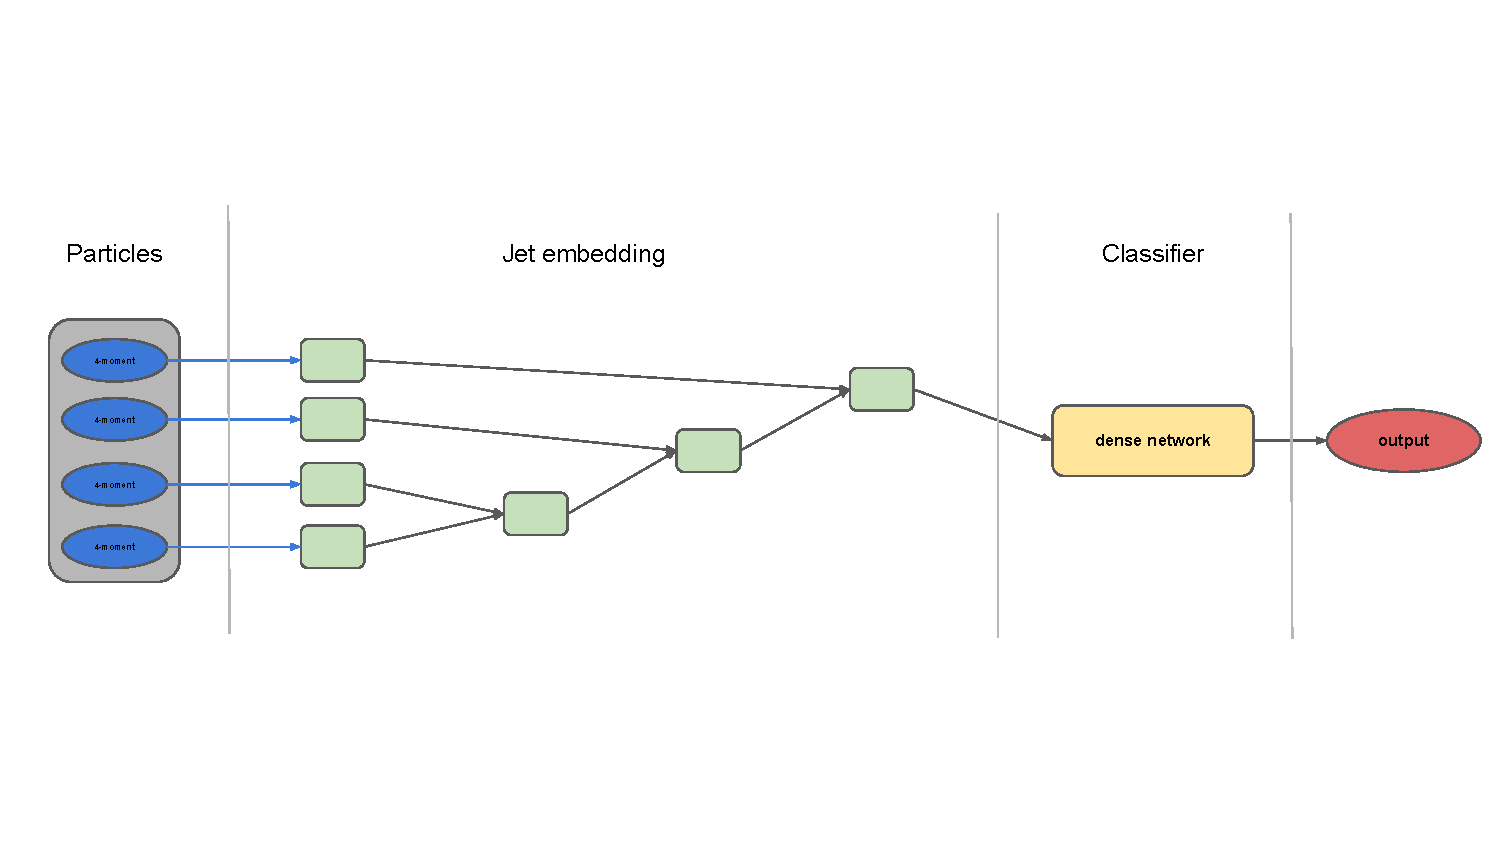
\includegraphics[width=\textwidth]{Images/RecNN_diagram_not_parall.pdf}
    \caption{Diagram of the overall node structure of the gated RecNN. The order in which the node are merge is determined by the chosen jet clustering metric. Every green unit represent the evaluation of the same unit. The black arrows in this diagram represent the flow of both the 4-momentum and the embedding array, meaning it represent both black and blue arrows from the node diagrams.}
    \label{fig:recursive_network}
\end{figure}


Similarly to how RNNs were designed to fit the needs of language processing, another architecture type has been designed to fit the needs of jet classification. This architecture type, called recursive neural network (RecNN), was devellopped following the idea behind jet clustering, and applying such architectures to the problem of boosted W-jet tagging \cite{Louppe:2017ipp}.

\subsection{Architecture}

As in a RNN, the network architecture is divided into two parts, a jet embedding part and a final classifier made from a dense neural network. Contrarily to the linear structure of the sentence embedding, the embedding part is organised from a jet clustering structure. The 4-momentum of each input particle is fed into a version of the unit design to only take a particle as input, those units iterations are called leaf nodes. Then two nodes are selected from the clustering metric and their output is fed into an inner node, designed to now take two nodes output as inputs. This process is repeated, still using the clustering metric at each step to determine which two nodes are to be merged into a new node next, until only one node remains, as illustrated in Figure \ref{fig:recnn_architecture}. The output of the final node is finally fed to the classifier part to provide a final output. 
The metric used to select which nodes are to be merged can be chosen among the following set:
    
\begin{itemize}
    \item randomized : two nodes are selected at random
    \item pt-ordered : the nodes holding the two pseudo-particles with the highest pt 
    \item reversed pt-ordered : the nodes holding the two pseudo-particles with the lowest pt
    \item $k_t$ : nodes holding closest pseudo-particles following the kt clustering metric
    \item Cambridge : nodes holding closest pseudo-particles following the Cambridge clustering metric
    \item anti-$k_t$ : nodes holding closest pseudo-particles following the anti-kt metric
\end{itemize}
The distance of two particles $i$ and $j$ in a clustering metric is defined as
\begin{equation}
    d_{ij} = \mathrm{min}(p_{Ti}^{2k},p_{Tj}^{2k}) \frac{\Delta_{ij}}{\mathrm{R}} \mend
\end{equation}
In this expression $\Delta_{ij}$ corresponds to the distance of the particles in the ($\eta$,$\phi$) plane, R is a distance parameter, and $p_{Ti}^{2k}$ corresponds to the modulus of the transverse momentum of particle $i$, with the $k$ parameter taking a value of 1 for the kt metric, 0 for the Cambridge metric, and $-1$ for the anti-kt metric.

In the jet embedding part, the information actually takes two parallel paths. For each inner nodes, the 4-momentum of the particle or pseudo-jet of the two merged nodes is added. This new pseudo-jet is both used in the change of the embedded representation array and then propagated as secondary input to the next merge.

\subsubsection{Node layout: gating}


\begin{figure}
    \begin{center}
    % \subfloat[RecNN leaf]{
        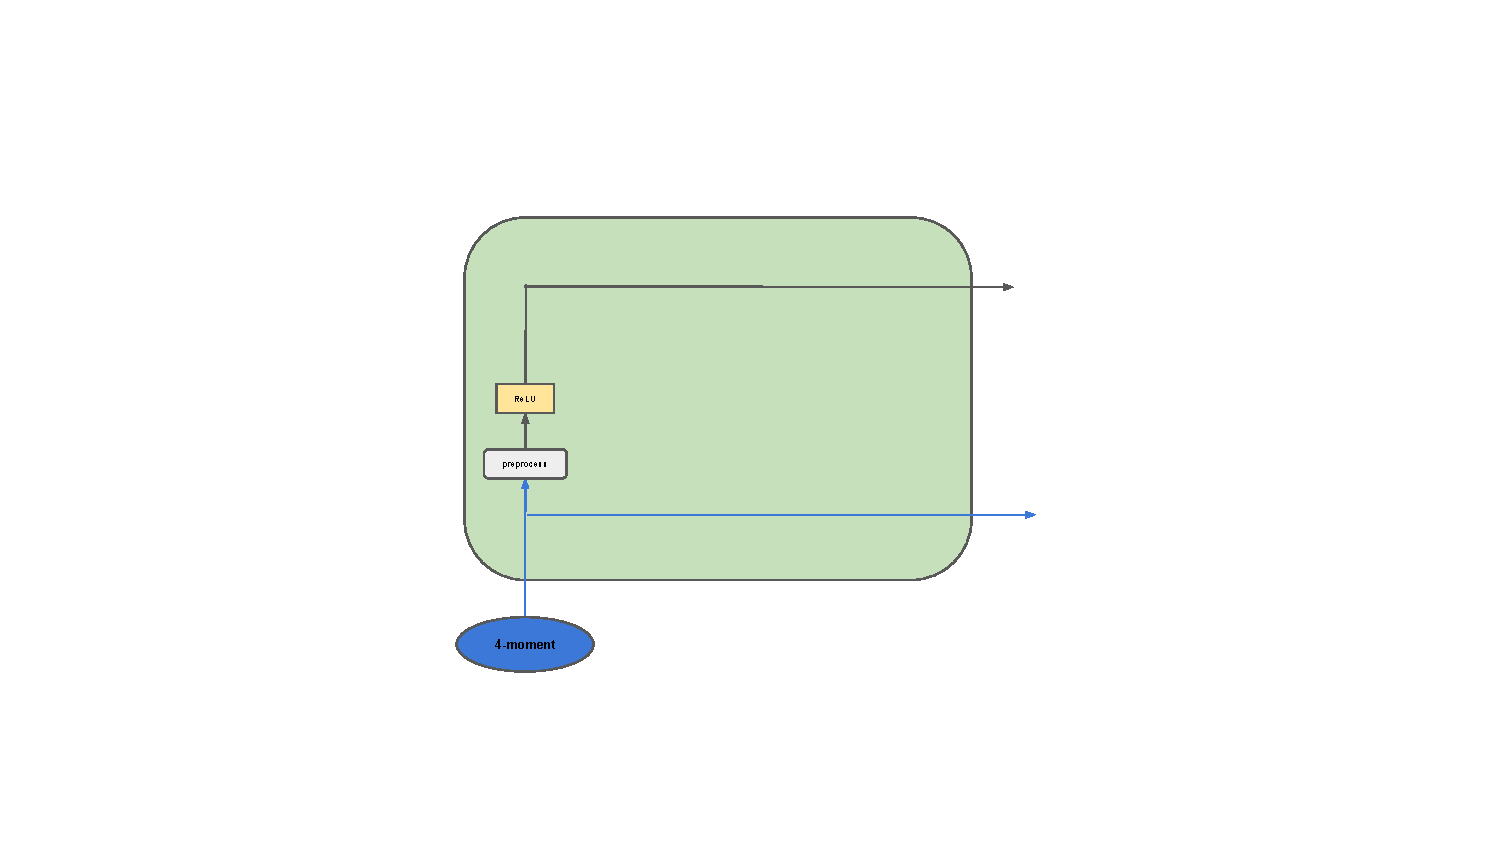
\includegraphics[width=\textwidth]{Images/Schema_RecNN_Leaf.pdf}
        \label{sub:RecNNLeafNode}
    % }
    
    % \subfloat[RecNN node]{
        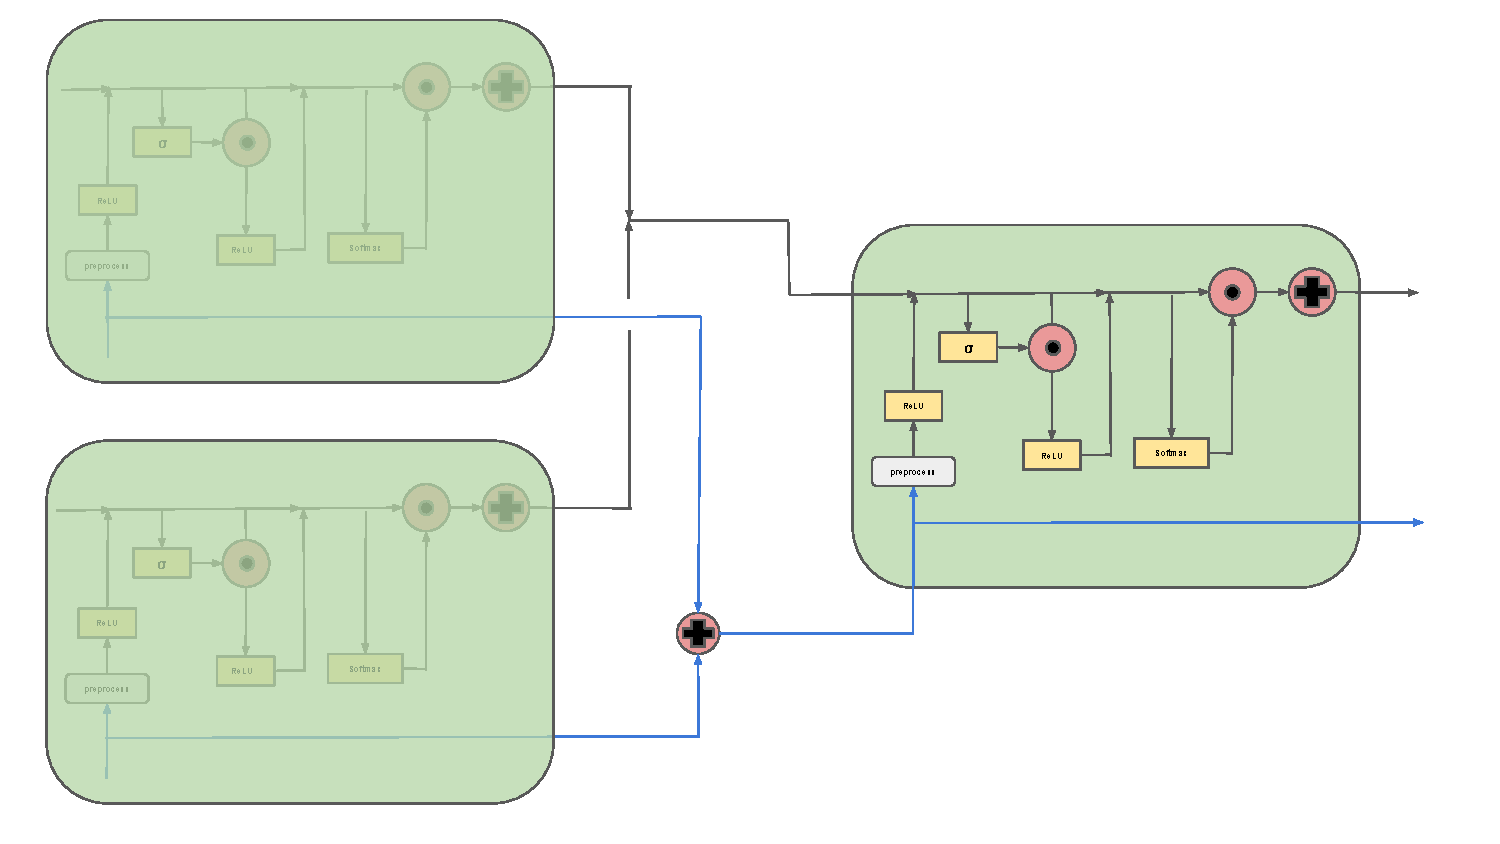
\includegraphics[width=\textwidth]{Images/Schema_RecNN.pdf}
        \label{sub:RecNNNode}
    % }
    
    % \subfloat{
    %     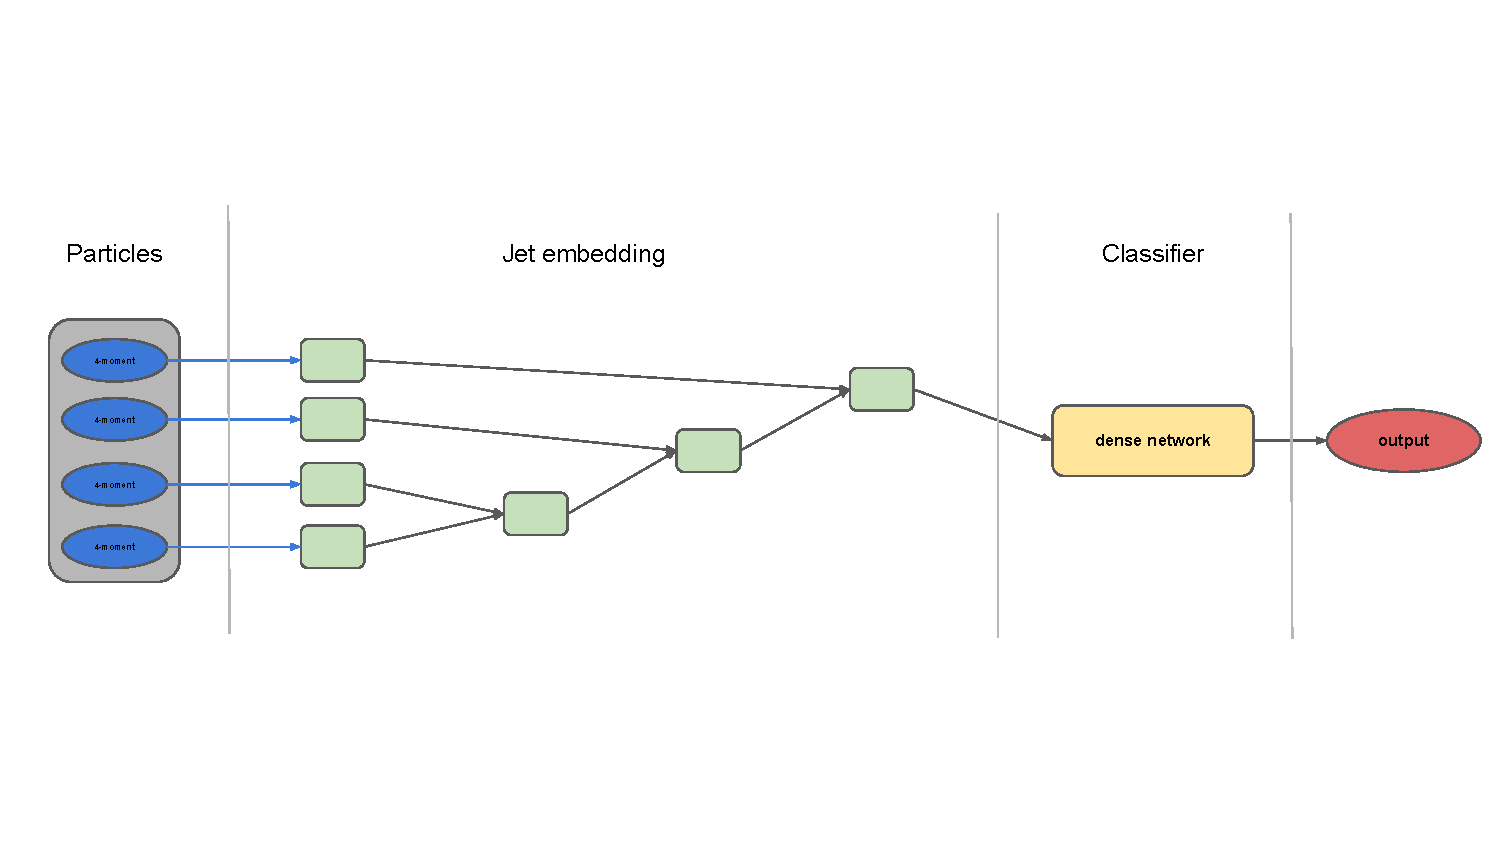
\includegraphics[width=\textwidth]{Images/RecNN_diagram_not_parall.pdf}
    %     \label{sub:RecNN_full}
    % }
    
    \caption{Diagrams of the nodes that can be found in a RecNN architecture. The top is a leaf node, meaning directly taking a particle 4-momentum as only input. Bottom illustrates the inner structure of a node as well as how its input are taken from the previous nodes. The green boxes represent several iteration of the same unit. The yellow rectangular boxes represent a single neuron layer, and their names correspond to the activation function of the neurons in that layer. The blue arrows represent the path of 4-momentum merging at each iteration. The black arrow represent the path of the embedding arrays. the plus and dot signs in the red circles represent element-wise sum and element-wise product respectively. The white box represent a preprocessing step that involves the transformation into cylindrical coordinates, as well as a scaling of each variable. More information on these operation can be found in the text.}
    \label{fig:recnn}
    \end{center}
\end{figure}

While several node layouts are tested in \cite{Louppe:2017ipp}, the gated layout has the best results and is the basis of our version. Inspired by the long short-term memory (LSTM) architecture \cite{lstm} and gated recurrent unit (GRU) architectures \cite{GRU}, the gating conceptually adds the possibility for the network to select and mix available information more easily. While a mathematical formulation of this layout is available in the appendix of the article, the following explanation relies on the illustration in figure \ref{fig:recnn_nodes}. 

First, each leaf node takes the 4-momentum of a particle and directly propagate it as its secondary output. A copy of this 4-momentum is pre-processed, which consists in two distinct steps. The first step is changing the expression of this 4-momentum from the easily addable Cartesian coordinates, to the more interpretable cylindrical coordinates. A few more variables are also computed at this step, like the 3-momentum modulus and the mass. Each of those variables are then scaled by the robustScaler method \cite{robustscale} trained on the whole dataset. The goal of this scaling is to allow the distribution of each of the variables to be comparable with one another in terms of median and quantiles, conceptually avoiding the following layers to have to learn the scales of each variable. 

The output of this pre-processing step is then given as input to a ReLU layer, which output array, designed to be of the same shape as each of the concatenated embedding arrays, is also concatenated with the embedding outputs of the previous layers. A new ReLU layer is evaluated by combining the information in this new embedding array using a reset gate. Conceptually, the goal of this reset gate is to actively select which parts of the embedding array are to be emphasized, and which parts are to be forgotten. This reset gate is implemented by the use of a sigmoid layer, taking as input the embedding array and creating a same-shaped output array of values between 0 and 1. An element-wise product between the output array and a copy of the embedding array is then computed before feeding the produced array into the ReLU layer. The output of the ReLU layer, designed to have the same shape as each concatenated array, is then also concatenated to the embedding arrays.

At this point the embedding array consist of the concatenation of four different arrays of the same shape: two embedding arrays outputs from the previous nodes, a local evaluation of the pseudo-jet and an array produced from the combination of all the previous ones. In order to combine all those information into an array of the desired shape, a softmax gate is applied. This softmax gate has the goal of weighting each variable of the embedded array by a scalar, before the four concatenated arrays are added element-wise. The weights are determined by a softmax neuron layer. The output weights $w_i$ of this softmax layer is determined from the activation of each output neuron $Z_i$ by
\begin{equation}
    w_{i} = \frac{e^{Z_i}}{\sum_{j=1}^{K}e^{Z_j}} \mend
\end{equation}
The product of this softmax gate is then the embedding array output of this node. If the node is the final node, this output is then directly fed into the dense neural network classifier part of the architecture.

\subsubsection{Pre-processing}

In order to simplify the task, jets are de-boosted and centered using the highest \pt particle, meaning particles appear orientated around the center (0,0) of the ($\eta$,$\phi$) plane. The jet is then re-clustered into three subjets and rotated and even mirrored so that the general disposition of subjets appear similar. This is done in order to simplify the task for the network, as the orientation of the jet in the detector is not considered relevant for this task.

\section{Recursive neural network for hadronic tau decay identification}


\begin{figure}
    \centering
    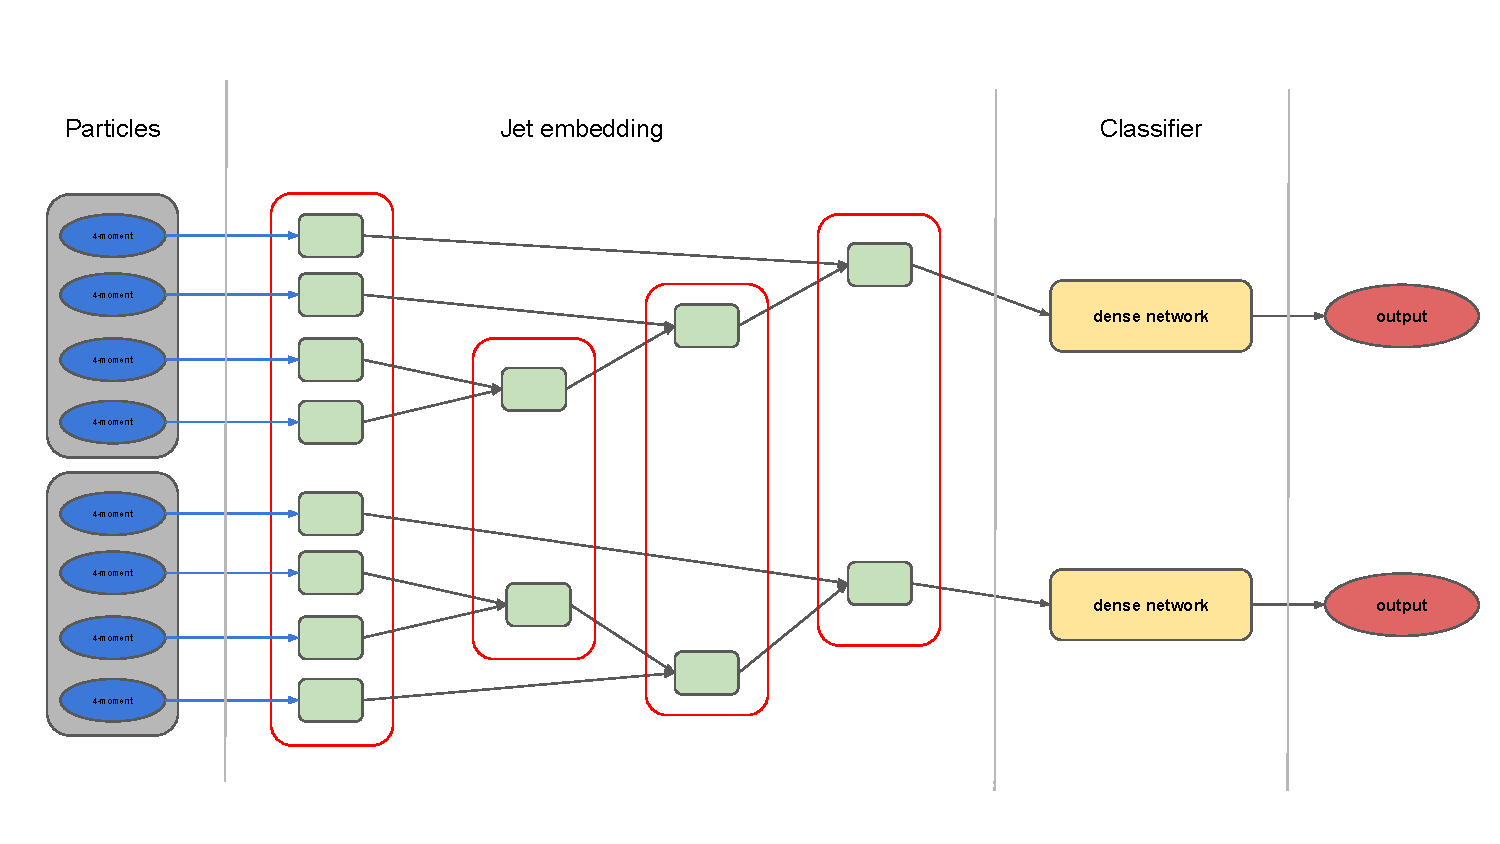
\includegraphics[width=\textwidth]{Images/RecNN_diagram_parall1.pdf}
    \caption{Illustration of the parallelisation of computing in the RecNN. The red boxes correspond to node-depth levels that are evaluated and trained simultaneously in a single mini-batch.}
    \label{fig:RecNN_parall}
\end{figure}



\subsection{Implementation}

While most neural network architectures can easily be implemented using widely available libraries, the nature of the RecNN architecture, mainly its changing structure that adapts to each jet, is not implemaentable from these libraries. The RecNN architecture was therefore implemented by the authors of \cite{Louppe:2017ipp} using basic classes from the sklearn library \cite{scikit-learn}. Therefore, the implementation shared by the original article \cite{Louppe:2017ipp} was used as a base for our own implementation. 

The first difference brought by our implementation is purely an optimisation of the code. While the code was already designed to be run in parallel on several cores at the evaluation and training phases, the pre-processing steps were not. By adapting those steps and running in parallel the time needed for this step was significantly reduced. Time was also gained by changing the format under which the arrays were saved on disk.

In order to compare the different methods and to study population effects, the code was adapted to be able to track jets through the evaluation process. Indeed, in the original code the formatting of particles into the arrays used as input to the RecNN meant the loss of its link with any other information, such as the score of the jet with the standard technique, or the gen-level information. This tracking also allowed to build a display of jets with their associated gen-level information, allowing a case-by-case study.

\subsection{Upgrade}

In the original implementation, particles are described only by their 4-momentum. But the nature of those particles as well as other available information is not used in this process yet. In order to add this information, the 4-momentum was changed to an array holding extra information. From the layout of a node, as illustrated in Figure \ref{fig:recnn}, this extra information must therefore consist of variables that can be added at each merging of two nodes.

The first variables added are the energy contributions from each particle type, namely photons, electrons, muons, charged hadrons and neutral hadrons. In the case of charged particles, these contributions are also split each into two different contributions depending whether their trajectory is found to be displaced from the original vertex ($\Delta z < 0.2\,\mathrm{cm}$). 

The decay modes of \tauh can only give a one or three charged hadrons and eventually a few photons in the final state. With this in mind the number of particle of each type is also added, as it is naturally considered a important information that the network was missing so far.

\subsection{Performance}

\begin{figure}
    \centering
    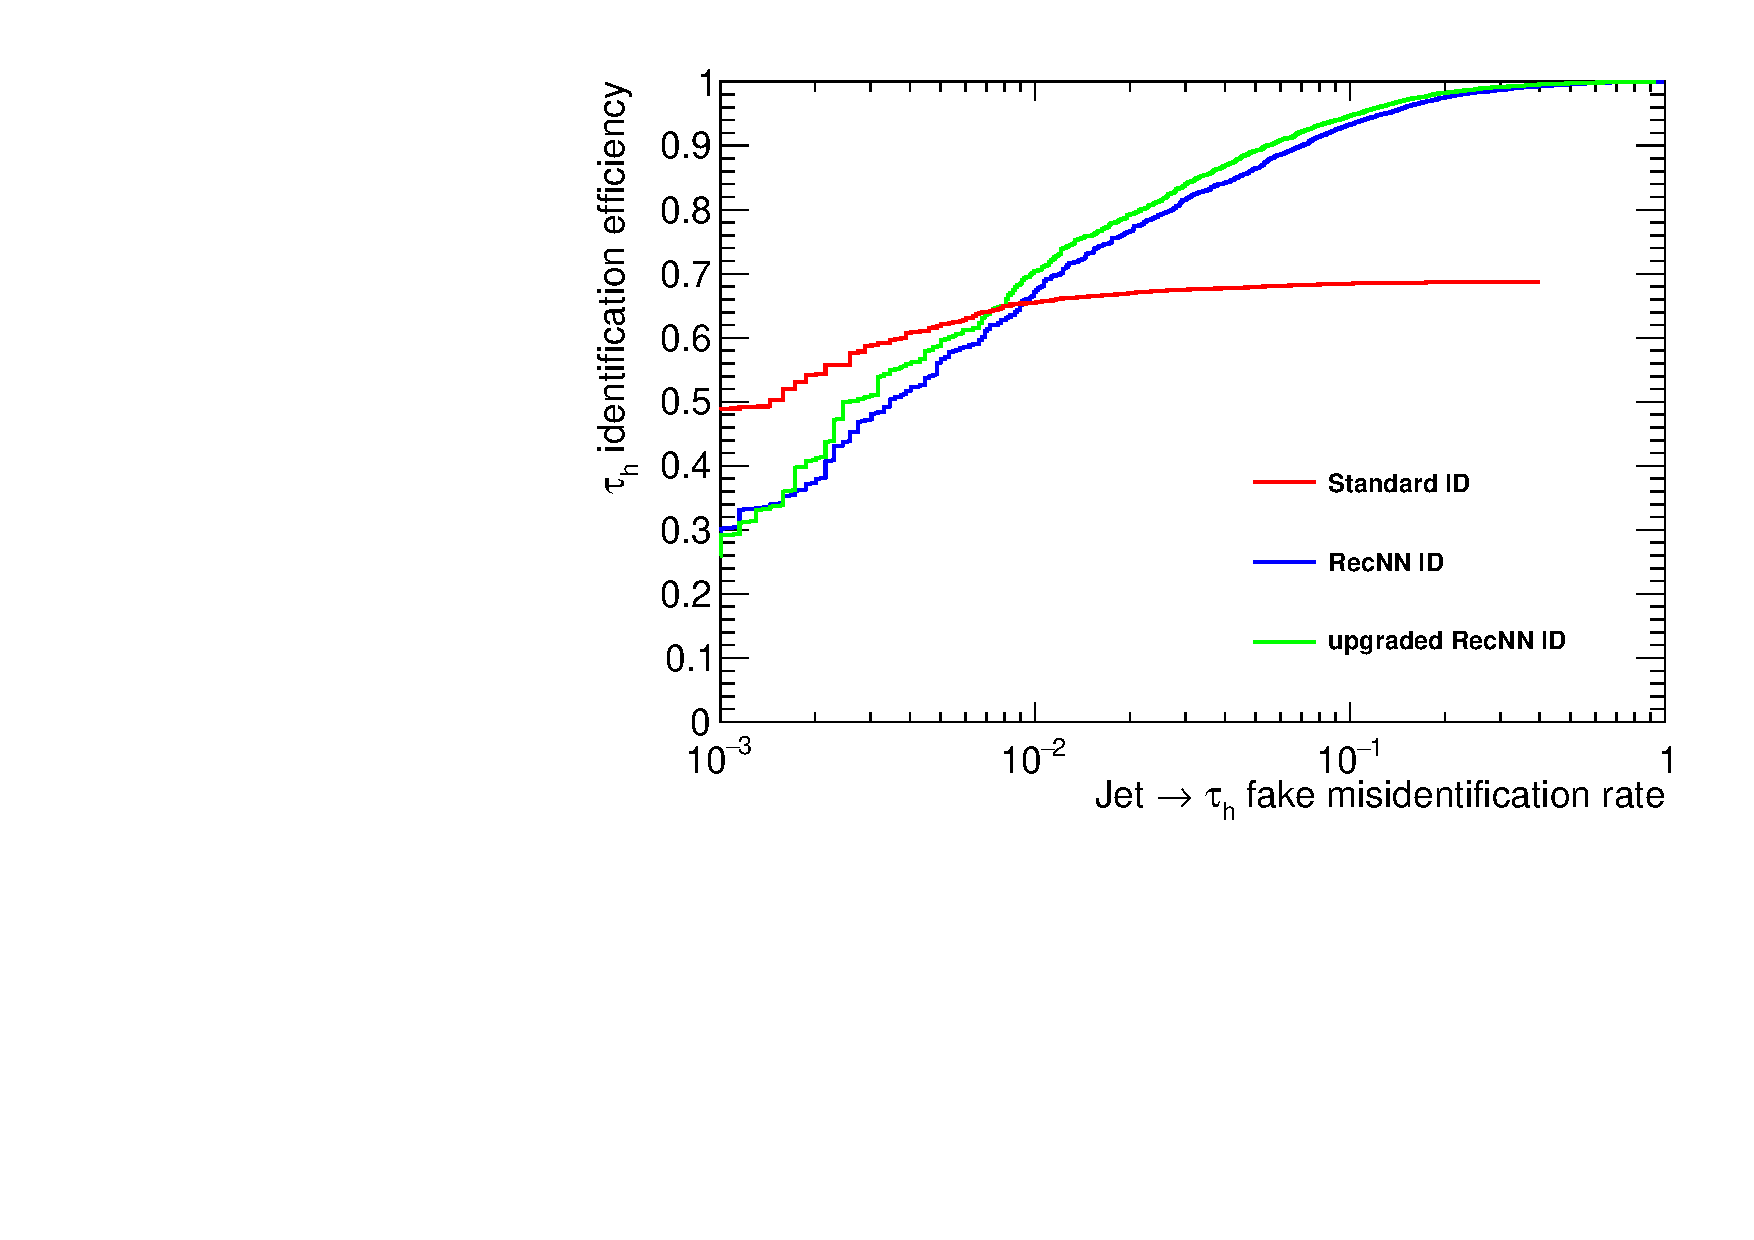
\includegraphics[width=\textwidth]{Images/ROC_comp_all.pdf}
    \caption{\tauh identification ROC curve for the standard method and with the RecNN method. The x axis is set to a logarithmic scale.}
    \label{fig:RecNN_ROC}
\end{figure}

The ROC curves of both the standard method, the base RecNN implementation and the upgraded RecNN approach are presented in figure \ref{fig:RecNN_ROC}. While the area under the curve is strictly better in the RecNN approaches compared to the standard method, the efficiency of the standard method is still better at low jet misidentification rate. The gain from the upgrade of the RecNN, while significant, is less than expected. 


\subsection{Possible optimisation}

Although the results have shown some potential, this study has not reached the level of optimisation that could help the RecNN to outperform the standard technique systematically. Indeed, several upgrades that could benefit the RecNN approach have been considered, but where not fully implemented in time. 

Even while limiting as much as possible the computational times, the latest versions of the RecNN network have proven to be long to train, about two days on a dedicated machine with 40 cores. All the clustering orderings have shown similar results in several stages of optimisation. While all should be optimised and tested in time, the presented results have been produced with the anti-$k_t$ ordering.

One such upgrade idea come from the study of QCD jets misidentified by the RecNN. Indeed, many examples such as the QCD jet mistagged as a \tauh by the RecNN network displayed in figure \ref{fig:jet_display} show that the RecNN approach does not use the number of particle information as efficiently as it could. An upgrade would be to directly add the number of particle per type at the classifier-level, rather than the jet embedding level. This could help the network to easily reject trivial cases, while being able to specialize the jet-embedding part for the less straight-forward cases.

In our training sample, a majority of training cases are trivial, meaning most of the cases will not help the network to learn the classification requirements of the difficult cases. While this could be mitigated by re-training more times using the training samples, the re-use of a training sample many times come with a problem called overtraining. This problem comes when the networks learns discrimination characteristics that are specific to the training sample, and not generalisable. To avoid this overtraining, the training phase is stopped when the evaluation of the network on an independent sample starts showing a worsening performance, while the performance on the training sample keeps getting better. A possible upgrade could then be the use of a selected subset of QCD jets in the training, specifically jets that are similar to \tauh. A part of other jets should still be present in the selected sample, as not to lower the rejection efficiency on those jets, but should take a less important part of the training sample. 

While all those optimisations were attempted, these were not implemented in time. The RecNN approach has shown good performances already, and while the upgrades have improved these performances, further improvements are expected from the study on a case-by-case basis. The potential optimisation that were discussed could help reach new performances.

\begin{figure}
    \centering
    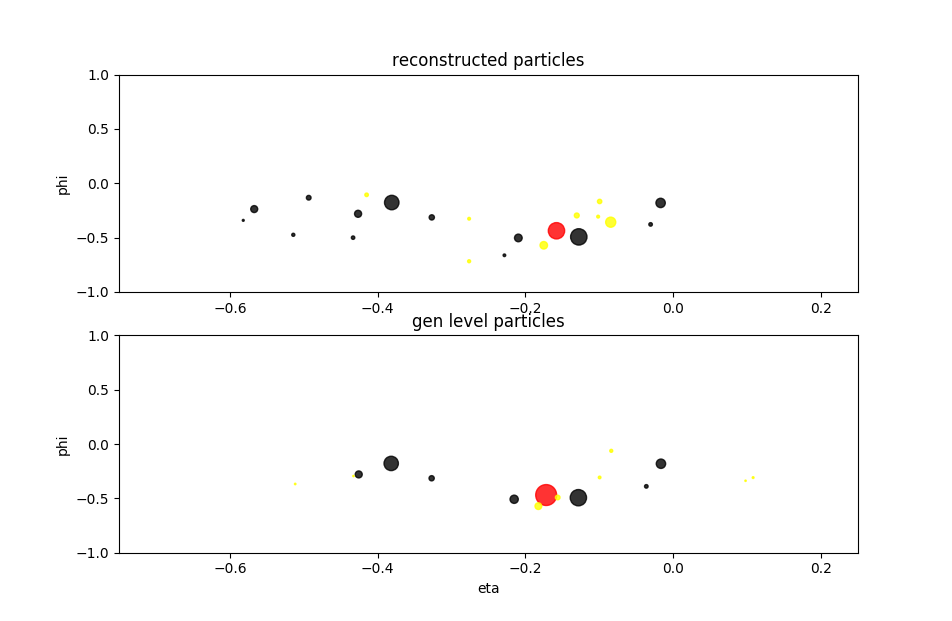
\includegraphics[width=\textwidth]{Images/display.png}
    \caption{Scatter plots of the constituents in a QCD jet misidentified by the RecNN network. Top plot is the reconstructed jet, and the bottom plot is the gen-level jet. The size of the points are proportional to their \pt and their color depends on their type. Black is a charged hadron, yellow is a photon and red is a neutral hadron.}
    \label{fig:jet_display}
\end{figure}
    
% % LSTM
%     \chapter{LSTM}
%     \textcolor{red}{This chapter covers three areas: analysis of the data; discussion of the results of the analysis; and how your findings relate to the literature. The analysis of the data can be discussed here but the details of any analysis, such as statistical calculations, should be shown in the appendices. You should present any discussion clearly and logically and it should be relevant to your research questions/hypotheses or aims and objectives. Insert any tables or figures that you decide are important in a relevant part of the text not in the appendices, and discuss them fully. Make sure that you relate the findings of your primary research to your literature review. You can do this by comparison: discussing similarities and particularly differences. If you think your findings have confirmed some literature findings, say so and say why. If you think your findings are at variance with the literature, say so and say why.}
\section{Results}
Lorem ipsum dolor sit amet, consectetur adipiscing elit. Duis ut ipsum nec orci interdum sollicitudin ut eu nunc. Pellentesque ultricies eros in justo sagittis, eget blandit velit aliquet. Aenean ac lectus nibh. Quisque ac est pellentesque, ullamcorper sem sit amet, pharetra quam. Morbi ullamcorper placerat diam, sed tincidunt odio.

\textcolor{red}{When placing tables (\autoref{tab:econ}) within the body of the text, the citation is placed above the table.} 

\begin{table}[!ht]
  \centering
  {\small {\it \caption{The economic argument \label{tab:econ} \hcite{econ}}}}
  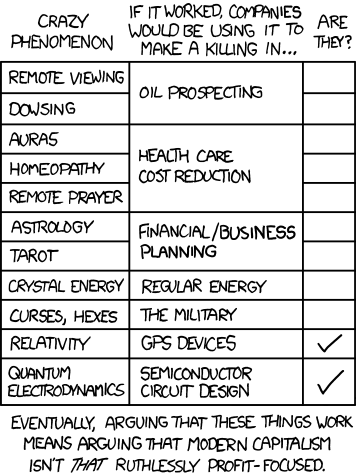
\includegraphics [scale=0.5]{Images/the_economic_argument.png} \\
\end{table}

\vfill

\newpage 

\section{Discussion}
Lorem ipsum dolor sit amet, consectetur adipiscing elit. Duis ut ipsum nec orci interdum sollicitudin ut eu nunc. Pellentesque ultricies eros in justo sagittis, eget blandit velit aliquet. Aenean ac lectus nibh. Quisque ac est pellentesque, ullamcorper sem sit amet, pharetra quam. Morbi ullamcorper placerat diam, sed tincidunt odio.

\textcolor{red}{When placing figures (illustrations, pictures, graphs, diagrams, charts, maps etc.) within the body of the text, the citation is placed below the figure (\autoref{fig:moun})}

\begin{figure}[!h]
  \centering
  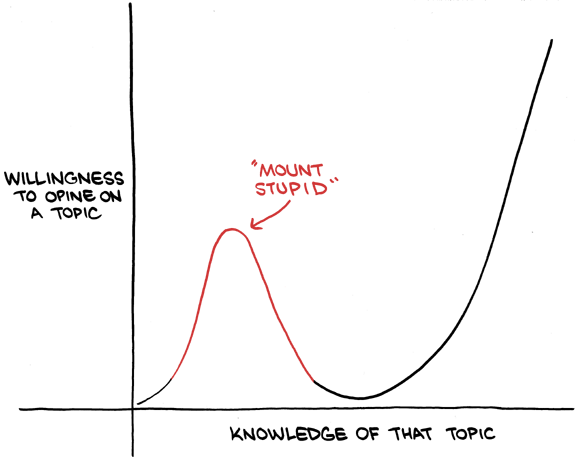
\includegraphics [scale=0.5]{Images/dunning_kruger.png} \\
  {\small {\it \caption{Dunning–Kruger effect \label{fig:moun} \hcite{mount}}}}
\end{figure}
    
% Search for a MSSM heavy Higgs boson
    \chapter{Search for a MSSM heavy Higgs boson}
    This chapter describes the search for a neutral MSSM Higgs boson through its decay to a pair of hadronically decaying tau leptons ($H \rightarrow \tauh\tauh$). Both CMS and ATLAS collaborations have discovered the decay of the Standard Model Higgs boson into a pair of $\tau$ \cite{ATLASHtt,CMSHtt}. In the context of the MSSM, three neutral Higgs bosons are predicted: the CP-even states h and H and the CP-odd state A, which may all decay to $\tau$ pairs. A model-independant search for a single Higgs boson, denoted $\Phi$, is performed in a $m_A$ in the range 90 GeV to 3200 GeV. The analysis is sensitive to production via gluon-gluon fusion and production in association with b-quarks. The cross section of the latter increases for larger values of $\mathrm{tan}\beta$ due to the enhanced down-type fermion Yukawa couplings.  The search is also performed in the $m_A - \mathrm{tan}\beta$ parameter space of the $m_{h}^{max}$ scenario \cite{Carena2003} for the same mass range.

Searches for MSSM neutral Higgs bosons have been performed by the collaborations at LEP \cite{Schael2006}, the Tevatron \cite{Benjamin:2010xb}, and at LHC by the CMS and ATLAS collaborations \cite{Aaboud2018,Sirunyan2018} with no excess observed above the background expectation. 

The results presented here follow those published by CMS in 2018 but makes use of the new 2017 data while being restricted to the \tauh\tauh channel, corresponding to an integrated luminosity of 41,5 $\mathrm{fb^{-1}}$. Event categorisation is used to enhance sensitivity to particular production modes. The production of neutrinos in the tau decay makes it difficult to reconstruct the invariant mass of the candidate Higgs boson. Statistical inference is therefore performed on the distribution of the $m_{T_{total}}$ variable, designed to give a better signal to background separation from the presence of neutrinos, and therefore \MET in signal events.

Section \ref{sec:analysis_samples} outlines the collisions datasets of real data, defined by which trigger those collisions fired, and MC simulation, defined by which hard process was generated. The event selection is then detailed in section \ref{sec:analysis_eventsel} which is done in a framework partially developed for this purpose. The estimation of each background process, using data-driven methods where possible, is detailed in section \ref{sec:analysis_background_methods} and followed by a summary of the experimental and theoretical uncertainties affecting the signal and background estimations in section \ref{sec:analysis_systematics}. The statistical procedure used to quantify the presence of signal in the data is given in section \ref{sec:analysis_statistical_interpretation} and is followed by the results of the search in section \ref{sec:analysis_results}.

\section{Data samples and simulation}
\label{sec:analysis_samples}

\subsection{Data triggers}
Real data datasets are defined by which trigger pattern they were gathered from. Events are therefore selected by dedicated trigger algorithms, which in our case require the appropriate pair of \tauh objects. An additional single high \pt \tauh trigger was added to improve sensitivity in the high \pt region. At the HLT level, defined in section \ref{sec:trigger}, the di-\tauh triggers require two HLT-\tauh objects to be identified and not to overlap. For this a simplified version of the PF algorithm is run for both \tauh reconstruction and isolation. The isolation requirement is designed to be loose with respect to the analysis selection. The object properties determined in the trigger reconstruction, such as \pt and isolation, are only approximate to those in the full reconstruction. Consequently, the triggering of events that would pass the offline event selection is not fully efficient. The trigger efficiencies for \tauh candidates typically reach $60\%$ at the lowest \pt threshold of the analysis, and reaches a plateau of between $85\%$ and $95\%$ when around twice the \pt thresholds \cite{Sirunyan_2018}. 

In order to maximize the trigger efficiency for our analysis, asymmetric \pt threshold have been considered at the HLT level. The main concern of this study was finding a set of \pt threshold that would gain efficiency while keeping the firing rate at the same magnitude. 
In order to estimate those gains, both data and simulation had to be gathered without any \pt requirements. A new trigger pattern, which is similar to the classical double \tauh trigger but without any \pt requirements, was then implemented. The \pt requirements on the trigger-level objects were then applied offline on the \tauh trigger objects to simulate the new \pt thresholds.

To estimate the rate, the trigger pattern without \pt requirement was then applied to randomly selected collision events, to avoid pre-selection bias. The trigger rates are then evaluated by scanning the \pt requirement on each \tauh trigger objects. The rate was computed from the random selection rate as
\begin{equation}
    \mathrm{f} = \frac{n_{\mathrm{pass}}}{n_{\mathrm{total}}} \times \mathrm{f}_{\mathrm{unbiased}} \mend
\end{equation}
In this expression, $n_{pass}$ is the number of events that pass the trigger threshold, $n_{total}$ is the total number of events of the unbiased sample, and $\mathrm{f}_{\mathrm{unbiased}}$ is the rate of random selection used to produce the unbiased sample. 

This trigger pattern has also been applied to simulation events, from SM $H\rightarrow \tau\tau$ datasets, in order to determine the efficiency of these asymmetric triggers. The efficiency is computed as
\begin{equation}
    \epsilon = \frac{n_{\mathrm{trigger}}}{n_{\mathrm{selection}}} \mend
\end{equation}
In this expression, $n_{selection}$ is the number of events that pass the analysis requirements, and $n_{\mathrm{trigger}}$ is the number of these events that pass the trigger \pt requirements. This efficiency is then also scanned for different values of \pt requirements for each \tauh trigger objects.

While this study showed a gain of up to $6\%$ in efficiency by the use of asymmetric trigger thresholds, a $Z\rightarrow \tau\tau$ polarisation analysis showed the use of such a trigger pattern could reduce their acceptance of about $20\%$. The use of asymmetric \tauh trigger \pt threshold was therefore dropped.

\subsection{Simulation}
Several MC generators are employed to produce simulated samples of signal and background events. The MADGRAPH \cite{Alwall2011} matrix element generator is used for Z+jets, W+jets, $\mathrm{t\Bar{t}}$+jets and diboson production. To increase the number of simulated Z+jets and W+jets events passing the most signal-sensitive category selections, additional samples are generated with fixed jet multiplicity in the matrix element for up to four jets. These are combined with the inclusive samples by weighting events to maintain the cross-section ratios between jet multiplicity bins. The POWHEG \cite{Alioli2010} generator is used for single top-quark production. The SM gluon-gluon fusion and VBF production modes of the Higgs boson, treated as a background in this analysis, are also simulated with POWHEG at NLO precision. Production in association with a vector boson and both $ggH$ and $bbH$ MSSM modes are provided by PYTHIA \cite{SJOSTRAND2008852}. All samples utilise PYTHIA for parton showering and hadronisation and TAUOLA \cite{JADACH1991275} for tau decays. Additional proton-proton interactions are also simulated with PYTHIA and added to these events. The events are then weighted according to the number of these pileup interactions to match the distribution observed in data, as detailed in section \ref{sec:MC_corr}. 


\section{Analysis sequence}
\label{sec:analysis_eventsel}

This section describes the event-based analysis sequence, which goal is to select, correct and derives quantities such as weights and physical variables like \mttot, the final discriminating variable defined as 
\begin{equation}
    \mttot = \sqrt{m_{T}^2(\tauh^{(1)},\MET) + m_{T}^2(\tauh^{(2)},\MET) + m_{T}^2(\tauh^{(1)},\tauh^{(2)})}
\end{equation}
where
\begin{equation}
    m_T (x,y) = \sqrt{2\times \pt^x \times \pt^y \times (1-\mathrm{cos}(\Delta \phi_{x,y}))} \mend
\end{equation}
First, we will provide an overview of the framework partially developed and used for this analysis, called heppy. This will be followed by a description of the analysis sequence.

\begin{figure}
    \centering
    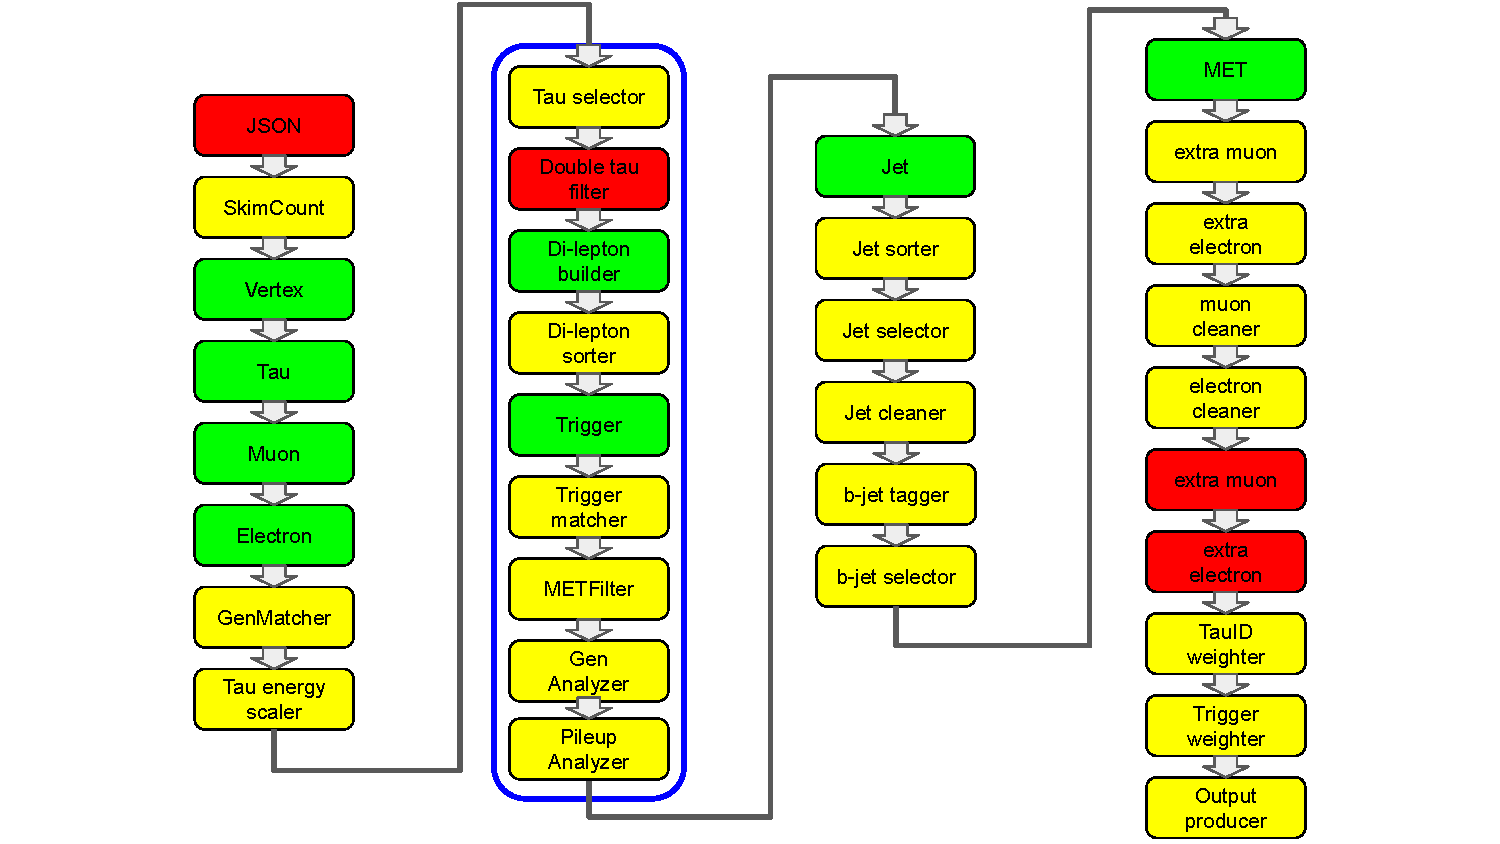
\includegraphics[width=\textwidth]{Images/HEPPY_diagram.pdf}
    \caption{Diagram of the selection flow implemented in heppy. Every box represents a module, called analyzer. Green analyzers create collections in the event instance by wrapping objects from the input in dedicated python classes. Yellow analyzers modify or compute a variable of the event. Red analyzers reject events that do not match given selection criteria. Finally, the blue highlighted section is the only part of the sequence that is specific to the \tauh\tauh channel. The rest of the sequence is used in other channels, like the semileptonic channels $e\tauh$ and $\mu\tauh$, and has been successfully tested.}
    \label{fig:HEPPY}
\end{figure}

Heppy is a python event processing framework for high energy physics based on ROOT. The inputs used in this analysis follow the MINIAOD format of the CMS collaboration. This format was design to hold the event-based information needed by most analyses. Therefore, the input files hold a lot of information, i.e. the lists of reconstructed physics objects, making it quite important in size, leading to sizeable computing times. Events are therefore selected by rejecting along criteria that are defined in the next sections, while also trimming the information that are not useful to our analysis, leading to a new light-weight format. Heppy is a modular framework, meaning all the processing is done in a feed-forward workflow with each step being encoded into a module called analyzer. Also physics objects retrieved from the ROOT files will be wrapped in python classes, allowing definition of useful methods and compatibility. Most analyzer of this workflow manipulate the defined physics objects to either create new useful variables, select subsets or reject events based on specific criteria. New sets of analyzers have been created in order to provide as much modularity and clarity as possible so that future analysis would be able to easily and promptly create this stage.

This section is focused on the desciption of the sequence for the \tauh\tauh channel. A diagram of the workflow developed is shown in figure \ref{fig:HEPPY}. In the order os usage in the analysis flow, the role of the analyzers are: 
\begin{itemize}
    \item JSON: Only active when running on real data. Rejects the events that have not been validated by the CMS collaboration.
    \item SkimCount: counts the number of generated events before selection. This is used later to renormalize the number of generated events to match the data integrated luminosity.
    \item Vertex/Tau/Muon/Electron: creates collections of the respective objects, and adds useful methods and attributes to these objects.
    \item Gen matcher: Only active when running on simulation. Matches reconstructed hadronic taus with closest generator-level particles, as described in table \ref{tab:mc_matching}.
    \item Tau energy scaler: only active when running on simulation, scales the energy of the taus, depending on their gen-level match. Stores the difference for eventual propagation to the \MET.
    \item Tau selector: first analyzer of the channel specific sequence, selects \tauh which have:
    \begin{itemize}
    \item $\pt > 40 \mathrm{GeV}$ and $|\eta| < 2.1$;
    \item passed the PF decay mode finding discriminator detailed in section \ref{sec:std_tau_id};
    \item  the distance between leading charged track and first primary vertex $d_z < 0.2 \mathrm{cm}$;
    \item passed the very loose working point of the anti-electron discriminator and the loose working point of the anti-muon discriminator. detailed in section \ref{sec:std_tau_id}.
    \end{itemize}
    \item Double tau filter: rejects the event if less than two \tauh fulfilling the requirements of the Tau selector have been found.
    \item Di-lepton builder: creates all possible combinations of two \tauh that have passed the selections, provided the \tauh:
    \begin{itemize}
    \item are separated by $\Delta R > 0.5$.
    \item have opposite-sign electric charges.
    \item both match the trigger objects associated with one of the HLT triggers within $\Delta R > 0.5$.
    \end{itemize}
    \item Di-lepton sorter: after these requirements there can be more than one candidate pair. In this case, the pair with the \tauh of highest \pt is chosen. If two pairs have the same \pt for their leading \tauh, the pair with the most-isolated highest \pt \tauh is chosen. In cse of more than one pair at this stage, the same criteria are then used on the second \tauh.
    \item Trigger: retrieves the trigger information
    \item Trigger matcher: checks if the selected \tauh pair matches the L1 trigger information.
    \item MET Filter: retrieves several flags that are provided by the CMS collaboration to reject events in order to mitigate several \MET reconstruction issues
    \item Gen analyzer: Only active when running on simulation. Retrieves generator level information in order to compute several weights, i.e the top quark and Drell-Yan \pt reweighting that are detailed in the next section.
    \item Pileup analyzer: Only active when running on simulation, retrieves pilup information and computes pileup weights, as detailed in the next section.
    \item Jet: creates collection of jets, and adds useful methods and attributes. Also applies the jet energy corrections as detailed in next section, while also storing the information for propagation to the \MET.
    \item Jet sorter: sorts the jet collection by \pt.
    \item Jet selector: jets are required to have $\pt > 30\,\mathrm{GeV}$ and $|\eta| < 4.7$, and to pass identification criteria to reject fake jets originating from detector noise, and pileup jets.
    \item Jet cleaner: discards jets overlapping with one of the two selected leptons, i.e. distance between jets and any lepton must be $\Delta R > 0.5$.
    \item b-jet tagger: applies the b-tagging scheme detailed in the next section.
    \item b-jet selector: creates a b-tagged jet collection from all jets passing the b-tag defined in the b-jet tagger, and of $|\eta|<2.5$.
    \item MET: retrieves \MET of the event. Applies all needed corrections and adjustments for previously corrected objects.
    \item extra muon (electron) cleaners: rejects events with any muons (electrons) passing a set of quality criteria, not considering the selected leptons in the semi-leptonic channels.
    \item TauID/trigger weighters: compute and apply the respective correction weights detailed in the next section.
    \item Output producer: Gathers all desired information and stores it in a flexible ROOT format allowing production of the distributions for statistical inference.
\end{itemize}

The output of this stage is used to perform a synchronisation with other CMS institutes working on the same analysis. For example a prototype of this sequence was used to synchronise on the previous MSSM search for a heavy Higgs bosons \cite{Aaboud2018} and helped figure out tweaks and upgrades in other group codes, and vice-versa. For this 2017 data analysis, a new synchronisation has been successfully performed.


\section{Background estimation methods}
\label{sec:analysis_background_methods}

For all processes apart from QCD multijet events, appropriate samples of MC simulation are available. While most background will be estimated by data-driven methods, these simulated samples are still used for a small part of the background contributions. Data-driven techniques not only tend to improve the data/MC agreement but also reduces the involved systematic uncertainties. Section \ref{sec:embedding} details how embedded samples are used to estimate $\mathrm{Z} \rightarrow \tau\tau$ events with two genuine tau lepton decays involved. And section \ref{sec:ff} describes how events where at least one of the tau candidates is faked by a jet are estimated by the fake factor method.

Monte-carlo simulated events (MC) are meant to provide an estimation of the contribution of processes that are not covered by the data-driven techniques. The data-driven techniques cover contributions based on the \tauh decay provenance. To distinguish the relevant processes that must be estimated from simulation, the reconstructed \tauh have to be matched to the generator particles available in the simulated samples. This is called referred to as gen matching. The exact definitions used to distinguish the different matched types can be found in table \ref{tab:mc_matching}.

\begin{table}[]
    \centering
    \caption{MC generator matching.}
    \begin{tabular}{|c|c|l|}
        \hline
        Value & Type & Generator level object properties \\
        \hline
        \multirow{2}{*}{1} & \multirow{2}{*}{Prompt electron} & $|\mathrm{pdgID}|==11$, $\pt > 8 \,\mathrm{GeV}$,\\
         & &  status flag IsPrompt \\
        \hline
        \multirow{2}{*}{2} & \multirow{2}{*}{Prompt muon} & $|\mathrm{pdgID}|==13$, $\pt > 8 \,\mathrm{GeV}$, \\
         & & status flag IsPrompt \\
        \hline
        \multirow{2}{*}{3} & \multirow{2}{*}{$\tau \rightarrow e$} & $|\mathrm{pdgID}|==11$, $\pt > 8 \,\mathrm{GeV}$,\\
         & &  status flag IsDirectPromptTauDecayProduct \\
        \hline
        \multirow{2}{*}{4} & \multirow{2}{*}{$\tau \rightarrow \mu$} & $|\mathrm{pdgID}|==13$, $\pt > 8 \,\mathrm{GeV}$, \\
         & & status flag IsDirectPromptTauDecayProduct \\
        \hline
        \multirow{2}{*}{5} & \multirow{2}{*}{$\tau \rightarrow \tauh$} & \multirow{2}{*}{Gen-tau jet} \\
         & & \\
        \hline
        \multirow{2}{*}{6} & \multirow{2}{*}{Jet/pu} fake & Anything that does not fall into \\
         & &  any of the above categories \\
        \hline
    \end{tabular}
    \label{tab:mc_matching}
\end{table}

The simulated background samples are split into three categories labeled T, J and L. T corresponds to events with gen match = 3, 4, 5 for both tau candidates. J corresponds to events with gen match = 6 for at least one of the hadronic tau candidates. L corresponds to all remaining events. In this analysis the T part of the background samples is replaced by the embedded samples and the J part is covered by the fake factor method. The remaining part is then covered by simulation.


\subsection{Monte-Carlo simulation}
\label{sec:MC_corr}

In order to mitigate the differences between data and simulations, several measurements have provided corrections that are applied in the analysis. These corrections are:

\paragraph{Pileup reweighting} MC simulated samples are generated with a given instantaneous luminosity which does not match the instantaneous luminosity of the data, which is often recorded after or during the production of the MC samples. In order to better fit the recorded pileup distribution in data a pileup reweighting is applied to MC events.

\paragraph{EE noise jets removal} Due to noise in the ECAL endcaps, all jets in a pseudo-rapidity gap of $2.65 < |\eta| < 3.139$ and of less than $50 \,\mathrm{GeV}$ are removed in both data and MC. The removal of the jet is also propagated to the \MET.

\paragraph{\tauh reconstruction efficiency} A data/MC scale factors (SF) is measured in $\mathrm{Z}\rightarrow\tau\tau$ events using a tag-and-probe approach. The selection of the tag-and-probe pairs is defined as follows. The tag \tauh must satisfy the kinematic, ID, and isolation requirements used in the analysis, in data it should also be matched to a trigger object. Probe leptons are only required to pass the kinematic cuts. Pairs of tag and probe leptons are considered when the leptons are same flavour and opposite sign charge, and are well separated ($\Delta R > 0.5$). The ID and isolation requirements used in the analysis are tested on the probe leptons, that can either pass or fail. The ID and isolation efficiency is defined as the number of passing probes divided by the total number of probes. The final efficiencies are extracted from a fit to the di-lepton invariant mass in the mass window around the $\mathrm{Z}$ mass. The scale factor applied to MC events is given by the ratio:
\begin{equation}
    SF = \frac{\epsilon(\mathrm{data})}{\epsilon(\mathrm{MC})} \mend
\end{equation}
For the embedded samples this scale factor is measured using a similar procedure. An additional correction is applied for embedded taus to correct for biases due to higher tracking efficiencies in embedded events than data. 

\paragraph{\tauh triggering efficiency} Trigger scale factors are also measured using a tag and probe method. For the trigger efficiency measurement, both the tag and the probe leptons must pass the ID and isolation requirements applied in the analysis, and passing probes are the ones firing the considered trigger. The efficiencies of the triggers are measured for data and MC. The scale factors for the double-\tauh trigger are measured in bins of the tau \pt, $\eta$, and $\phi$. Due to a bug in the embedded samples the efficiency of the tau triggers is significantly lower than the non-embedded SF. This bug affects some of the HLT requirements relating to the hadronic tau isolation cuts. To fix this issue the embedded taus are matched to earlier versions of the HLT \tauh objects before the problematic part. The scale factors are then used to cover the differences. The scale factors for the embedded samples use the same $\epsilon(\mathrm{data})$ measured for the MC scale factors but use the efficiency measured for the embedded taus in the denominator, the scale factor is then computed as:
\begin{equation}
    SF = \frac{\epsilon(\mathrm{data})}{\epsilon(\mathrm{embedding})} \mend
\end{equation}

\paragraph{Tau energy scale} The tau energy scale was measured using as observables the tau mass and the invariant mass of the system of the muon and the hadronic tau decay in $\mathrm{Z}\rightarrow\tau_{\mu}\tauh$ events. 

\paragraph{Jet energy} On top of the corrections detailed in section \ref{sec:jet_clustering}, corrections derived by the CMS collaborations to mitigate data/MC discrepencies are also applied \cite{collaboration_2011}.

\paragraph{Efficiency of lepton faking \tauh} Lepton can fake \tauh decay products, as their track can be misreconstructed as a charged hadron. The rates of such misreconstructions are measures by the collaboration and corrections are applied to simulation to match data expectation.

\paragraph{Lepton faking \tauh energy scale} A correction to the central values of the \tauh energies for \tauh candidates originating from electron (muon) fakes is applied for the 1-prong and 1-prong+1-\pizero decay-modes \cite{Chatrchyan2011}. 

\paragraph{Recoil corrections} Recoil corrections are applied to correct for the mismodeling of \MET in the simulated Drell-Yan, W+Jets and Higgs production. The corrections are measured on the vector $\Vec{U}$ defined as the vectorial difference of the measured missing transverse momentum and total transverse momentum of neutrinos originating from the decay of Z, W or Higgs boson
\begin{equation}
    \Vec{U} = \Vec{\MET} - \Vec{p}_{T,\nu} \mend
\end{equation}
The vector $\Vec{U}$ is projected onto the axes parallel ($U_1$) and orthogonal ($U_2$) to the boson \pt and it is measured in $\mathrm{Z}\rightarrow \mu\mu$ events, where the leptonic recoil does not contain neutrinos and the four-vector of the Z boson can be measured precisely. The effect of the recoil corrections on the \MET distribution of $\mathrm{Z}\rightarrow \mu\mu$ events, as measured by another CMS institute, is shown in figure \ref{fig:recoilcorr}.

\begin{figure}
\centering
\begin{subfigure}[b]{0.5\textwidth}
  \centering
  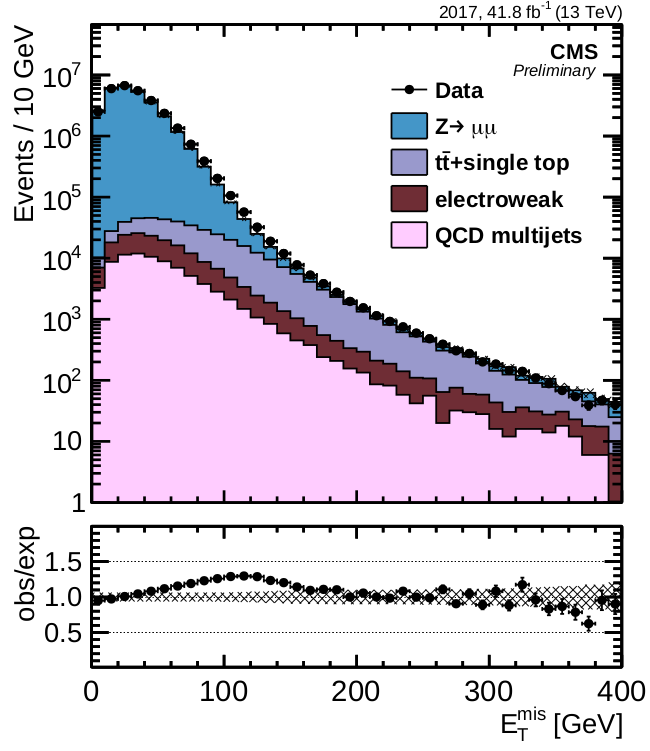
\includegraphics[width=\textwidth]{Images/withoutrecoil.png}
  \caption{\label{fig:recoil1} Without recoil corrections}
\end{subfigure}%
\begin{subfigure}[b]{0.5\textwidth}
  \centering
  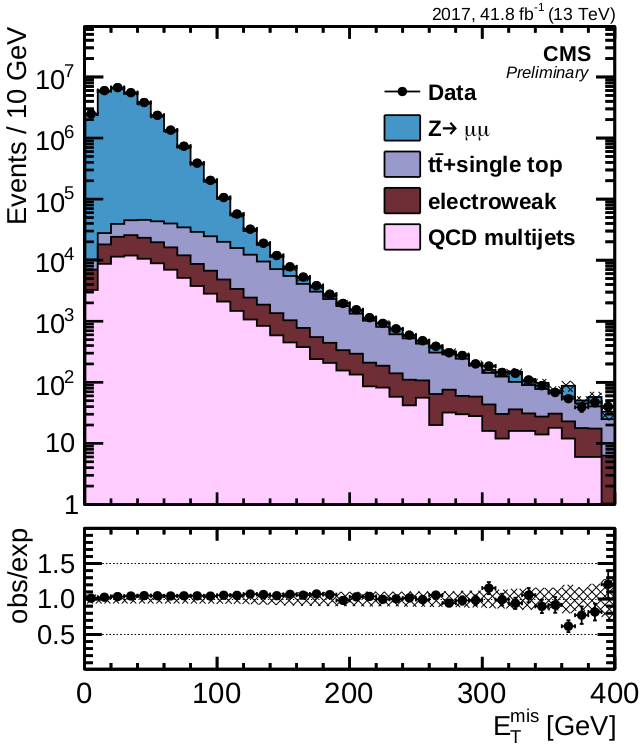
\includegraphics[width=\textwidth]{Images/withrecoil.png}
  \caption{\label{fig:recoil2} With recoil corrections}
\end{subfigure}
\caption{Effect of applying recoil corrections to the \MET distribution in the $\mathrm{Z}\rightarrow \mu\mu$ selection.}
\label{fig:recoilcorr}
\end{figure}

\paragraph{DY mass and transverse momentum reweighting} A reweighting is applied to Drell-Yan MC samples to correct the generator-level \pt and generator-level di-lepton mass distributions in LO madgraph samples. The correction is produced in a $\mathrm{Z}\rightarrow \mu\mu$ control region, as a function of the \pt of the $\mathrm{Z}$ and generator di-lepton mass to reduce the shape discrepancy between data and simulation. The weights are computed in such a way as to make the two-dimensional distributions of the $\mathrm{Z}$ \pt and the Z boson reconstructed mass match between data and simulation. The weights are then corrected not to introduce a general yield variation of the Drell-Yan background, but to only have a shape effect on the considered distributions. Those distributions before and after reweighting are shown in figure \ref{fig:DYreweight}.

\begin{figure}
    \centering
    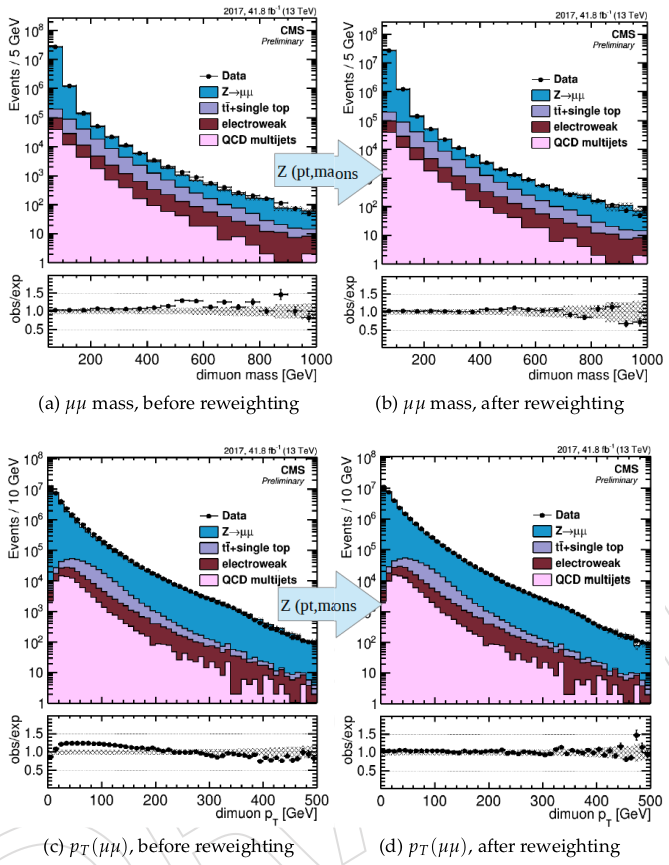
\includegraphics[width=.7\textwidth]{Images/DYreweight.png}
    \caption{Di-muon mass and \pt distributions in $\mathrm{Z}\rightarrow \mu\mu$ data before and after the reweighting.}
    \label{fig:DYreweight}
\end{figure}

\paragraph{Top quark transverse momentum reweighting} The modeling of the $t\Bar{t}$ background is improved by reweighting the \pt spectrum of the top quarks.

\paragraph{b-tagging efficiency} The efficiency for the tagging of b jets and the mistagging rate for light-flavour jets has been measured in both data and simulation. The efficiency and mistagging rate of the simulation is corrected through the application of efficiency and mistagging scale factors. The values of these factors and a description of the methods used to determine them can be found in \cite{Sirunyan_2018}. The simulation is corrected by randomly reclassifying, or demoting a fraction of tagged jets as untagged, or the other way around, i.e promoting, as necessary to result in the correct average efficiency and mistagging rate. The promotion or demotion probabilities for each jet are defined as
\begin{equation*}
    P(\mathrm{demote}) = 1 - SF \msep \text{when } SF < 1
\end{equation*}
\begin{equation*}
    P(\mathrm{promote}) = \frac{(SF-1)\epsilon}{\frac{SF}{\epsilon-1}} \msep \text{when } SF > 1 \mend
\end{equation*}
In this expression, the scale factor, $SF$, is $\pt$, $\eta$ and jet-flavour dependant ratios of data and simulation efficiencies, and $\epsilon$ is the measured tagging efficiency.

% \begin{figure}
%     \centering
%     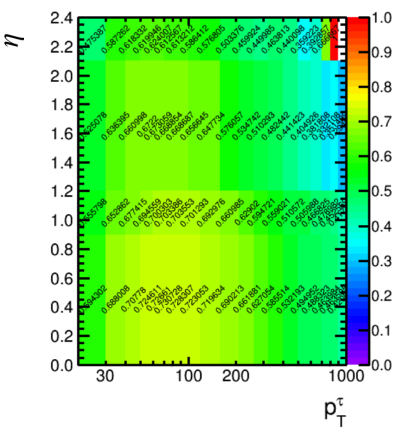
\includegraphics[width=.5\textwidth]{Images/btag_eff.png}
%     \caption{The b-tagging efficiency measured using $t\Bar{t}$ and DY MC in bins of b-jet $\eta$ and \pt.}
%     \label{fig:btageff}
% \end{figure}

\subsection{Embedding}
\label{sec:embedding}

The embedding technique allows an estimation of the standard model backgrounds with two taus in the final state from data, with minimal simulation input. A sample of di-muon events is selected from the recorded data. The two muons are removed from the event and replaced with simulated tau leptons with the same kinematic properties. In that way a set of hybrid events is obtained that relies on simulation only for the decay of the tau leptons. challenges in describing the underlying event or the production of associated jets in the simulation are avoided. A detailed description of the embedding technique can be found in \cite{CMS:2018apv}.

In this analysis, embedded samples are used in place of the MC simulated samples for $\mathrm{Z}\rightarrow \tau\tau$ and the parts of $t\Bar{t}$, di-boson and electroweak events where both tau candidates are matched to genuine taus at generator level.

\subsection{Fake factor method}
\label{sec:ff}
\begin{figure}
\centering
\begin{subfigure}[b]{0.5\textwidth}
  \centering
  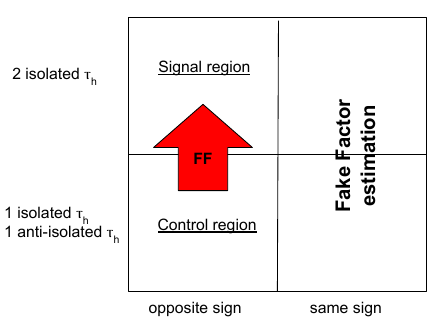
\includegraphics[width=\textwidth]{Images/FF_method.png}
  \caption{\label{fig:FF_method}}
\end{subfigure}%
\begin{subfigure}[b]{0.5\textwidth}
  \centering
  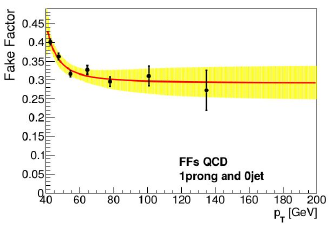
\includegraphics[width=\textwidth]{Images/FF_values.png}
  \caption{\label{fig:FF_values}}
\end{subfigure}
\caption{Illustration of the fake factor method. Diagram \subref{fig:FF_method} illustrate the way fake factors are measured, while \subref{fig:FF_values} illustrate some the values and fitted function used in the case of \tauh decaying to 1 prong and 0 jet in the event.}
\label{fig:FF_illustration}
\end{figure}

The fake factor method (FF) is used to predict all background sources with gluon- or quark-initiated jets misidentified as hadronic $\tau$ decays. The method is based on measuring the ratio of the number of events where preselected jets pass the \tauh ID criteria over the number of events that do not pass the ID criteria. Different regions are used to perform this measurement, depending on which background process is considered, namely QCD multi-jet, W+jets and $t\Bar{t}$. The preselection is defined by the same set of selection as the analysis, with the difference of a looser \tauh ID criteria, defining a region called the anti-isolated region. The value of the fake factor (FF) is then defined as
\begin{equation}
    FF = \frac{\text{passes preselection and passes \tauh ID discriminant}}{\text{passes preselection and fails \tauh ID discriminant}} \mend
\end{equation}
This fake factor is applied as a weight to events which pass the signal region selection except that the events are required to contain \tauh candidates satisfying the preselection criteria, but failing the nominal \tauh ID criteria (application region). The fake factor is estimated as a function of the jet multiplicity (0 or $\geq$ 1) and the \pt dependency is fit.

The fake factors are also determined separately for each of the channels $e\tauh$, $\mu\tauh$, and $\tauh\tauh$, accounting for differences in the selected background composition, the trigger requirements and in the \tauh ID criteria applied in each channel. For the \tauh\tauh channel, the determination region requirement is that the electric charges of the two hadronic $\tau$ candidates have the same sign. As for this channel the multi-jet background is by far the dominant fake \tauh background, the fake factors measured in the QCD determination region are also used to estimate any other backgrounds arising from fake \tauh.

The fake factor applied to a given event in the application region is a weighted average of the values measured for the different processes. The weight is given by the expected fraction of events of a given process in the application region. The weight is binned in $m_{vis}$ and number of jets. This weighted fake factor is applied to all events in the application region twice, once considering a \tauh as the fake, then considering the other as a fake, while multiplying both weights by $0.5$. Since genuine tau events in data are also present in the application region, the expected contribution from events with actual hadronic $\tau$ decays are subtracted using simulation. The expected fraction of events is estimated in two independent ways: via a template fit to the observed data, and via simulation. As the results of both methods agree and the template fit has convergence problems in some low-statistics event categories, the simulation-based estimate is used.

\section{Systematic uncertainties}
\label{sec:analysis_systematics}

This section describes the sources of uncertainty that affect the signal and background predictions of the \mttot distributions in each category. The experimental uncertainties typically concern either object selection or the methods to estimate the backgrounds described in the previous section, and are inherent to their respective measurement. The object selection is more important for the signal prediction, whereas the estimation methods have a large effect on the background estimation. Theoretical uncertainties affect the predictions of both signal and simulated background but are larger for the signal. Uncertainties can affect only the rate of signal, but some may affect both the shape and rate of the distributions. Each source of uncertainty will give a free parameter, called nuisance parameter, in the background estimation fit described in the next section.

\subsection{Shape uncertainties}

Most shape uncertainties, are evaluated by re-running the concerned simulated events through the workflow, but this time applying the up or down fluctuation on the considered variable. This leads to a multiplication of the overall computing needed to perform the full analysis, and is the main reason the semi-leptonic channels are not included in this analysis.

The following uncertainties cause variations in the shapes of the distributions.

\paragraph{Tau energy scale} Since the \mttot variable depends on the \pt of the selected \tauh, a separate shape uncertainty is applied for each decay mode in the simulated samples. In the embedded samples we have hybrid events where the simulated taus might be mixed with calorimeter deposits remaining from the removal of the original muons in the events. For this reason, the tau energy scale uncertainties for embedded samples are split into two parts, where $50\%$ are fully correlated with the uncertainty for fully simulated samples and $50\%$ are uncorrelated.

\paragraph{Jet energy scale} Since the change in jet energy is propagated to the \MET, the jet energy scale impacts the shape of the \mttot distribution. In general, the CMS collaboration derives uncertainties in the jet energy scale from 28 sources and combines them in a single uncertainty with one nuisance parameter. The uncertainty is split into several groups, instead of all 27 sources, because this would result in an unnecessary amount of parameters in the fit as well as a large technical effort. Instead, the sources are grouped according to the affected detector regions.

\paragraph{Energy scale of leptons faking \tauh} Shape uncertainties are applied to the \pt of the misidentified \tauh arising from the presence of leptons in MC samples uncorrelated between decay modes.

\paragraph{\MET unclustered energy uncertainty} The \MET takes into account the energy that is not clustered in the reconstruction process, impacting the value of \mttot. An uncertainty is therefore applied to all MC processes that do not have recoil correction applied.

\paragraph{\MET recoil correction uncertainties} For all MC processes that have recoil correction, uncertainties determined during the computation of the recoil corrections are propagated to the \mtot variable.

\paragraph{Top \pt reweighting} The uncertainty in the top \pt reweighting are estimated by not applying the correction and applying twice the correction in the $t\Bar{t}$ events.

\paragraph{DY \pt reweighting} The uncertainty in the DY \pt reweigthing are estimated by shifting of $10\%$ re-weighting applied to $\mathrm{Z}\rightarrow ll$ events.

\paragraph{B-tagging efficiency} The uncertainties in the b-tagging scale factors provided by the CMS collaboration are propagated to the the \mttot distribution in the categories defined by the presence or absence of b-tagged jets.

\paragraph{\tauh tracking efficiency for the embedded samples} An uncertainty in the tracking efficiency of hadronic taus in the embedded samples is propagated uncorrelated between 1 and 3 prong decay modes.

\paragraph{Fake-factor uncertainties} Uncertainties in the fake factor background estimation method consist of several sources:
\begin{itemize}
    \item Statistical uncertainty in the fake factor measurement in the control regions.
    \item Systematic uncertainties related to the QCD multi-jet fake factor corrections are propagated.
    \item Systematic uncertainties in the fraction of W/Z+jets events and $t\Bar{t}$ events with one misidentified \tauh in the anti-isolated region, adding two nuisance parameters. Those is evaluated by varying the fractions of those two background within uncertainties (including cross section and experimental uncertainties), while readjusting the fractions of the other processes to keep the sum at $100\%$.
\end{itemize}

\paragraph{Bin-by-bin uncertainties} To account for statistical shape uncertainties in the backgrounds due to the use of Monte-Carlo and embedded samples or templates derived from data events with limited number of events, we introduce shape variations to the background templates in all categories following the Barlow-Beeston approach, where the statistical uncertainties in each bin are used to define alternative shapes.

\subsection{Normalization uncertainties}

The number of events from each process is affected by a normalization uncertainty. A nuisance parameter following a log-normal distribution is applied on the yield of the affected process.

\paragraph{Luminosity} A $2.3 \%$ luminosity uncertainty is applied to the number of events predicted by pure Monte Carlo simulation \cite{CMS:2018elu}.

\paragraph{Tau ID efficiency} The uncertainty is applied to the number of events for all processes where the yield is estimated from MC, as well as the embedded events. Since two hadronic taus are required in the \tauh\tauh channel the magnitude of the uncertainty is $2.4\%$ for each \tauh, maning $5.5\%$ overall. The embedded samples also have an additional uncertainty applied to cover a tracking efficiency correction, with a magnitude of $2\%$ per \tauh.

\paragraph{Trigger efficiency} The uncertainty in the trigger efficiency amounts to $10\%$. The uncertainty is applied to all processes where the yield is estimated from MC, and to the embedded samples. The embedded and MC uncertainties are uncorrelated. In order to account for the efficiency of the double muon trigger that was used to select input events for the embedding technique, an additional $4\%$ uncertainty ($2\%$ per muon $= 4\%$) is applied to the embedded samples.

\paragraph{Background normalization uncertainty} A $4\%$, $5\%$, $6\%$ and $4\%$ uncertainty is applied to the $Z\rightarrow ll$, di-boson/single top, $t\Bar{t}$ and EWKZ processes, respectively, to account for the uncertainty in the production cross section of these processes. 

% \paragraph{Lepton to tau fake rate} Shape uncertainties were checked and no significant shape dependency has been observed in the event distributions used in this analysis. Therefore log normal uncertainties of $16\%$ ($26\%$) are applied for electron (muon) to tau fake rate.

\paragraph{Fake factor normalization} The uncertainty due to the subtraction of the genuine tau contribution is estimated by varying the substracted number of events by $\pm 10\%$, and amounts to about $2\%$ of the jet faking \tauh yield. %The fake factor shape uncertainties are normalized to the same area as the nominal shape, and the normalization factors are added in quadrature and act as separate nuisance parameters: this is done separately for the statistical uncertainties in the raw fake factors (about $5\%$) and the systematic uncertainties in the corrections (about $7\%$). Uncertainties are split in shape(-only) and yield uncertainties to capture the main variations induced by the uncertainties. This describes the two leading degrees of freedom of the fake factor \pt fits evaluated by toy experiments.

\section{Statistical interpretation}
\label{sec:analysis_statistical_interpretation}

This section outlines the statistical procedure used to quantify or reject the presence of a signal in data. These methods were developed by the LHC Higgs Combination Group to provide a common strategy for both the CMS and ATLAS Collaborations and to facilitate the combination of individual search results \cite{CMS-NOTE-2011-005}. 

The expected Higgs boson event yield in a given model can be denoted as $s$ and the background yield as $b$. This can refer equally to a simple counting experiment, or to predicted binned distributions for use in a shape-based analysis. An additional factor $\mu$ is introduced as a signal strength modifier, which allows for the signal rate to scale as $\mu \times s$. The background-only hypothesis is therefore defined by $\mu = 0$, and any signal hypothesis by $\mu > 0$. The term "data" will refer to an observed event count or counts, which could originate from an actual experiment or from simulation. The yields $s$ and $b$ are, in general, functions of nuisance parameters $\theta$ representing experimental and theoretical uncertainties. The nominal values $\Tilde{\theta}$ of these nuisance parameters are usually determined by external measurements, with uncertainties described by probability density functions $p(\Tilde{\theta} | \theta)$. From these components the likelihood for an observed dataset, $\Lagr(\mathrm{data}|\mu,\theta)$, is defined as
\begin{equation}
    \Lagr(\mathrm{data}|\mu,\theta) = \mathrm{Poisson}(\mathrm{data}|\mu\times s(\theta) + b(\theta)) \times p(\Tilde{\theta}|\theta) \msep
\end{equation}
where for a binned likelihood model the Poisson term is simply the product of Poisson probabilities over each bin $i$:
\begin{equation}
    \mathrm{Poisson}(\mathrm{data}|\mu\times s(\theta) + b(\theta)) = \prod_{i} \frac{(\mu s_i + b_i)^{n_i}}{n_i !} e^{-(\mu s_i +b_i)} \mend
\end{equation}

A ratio of likelihoods can be used to define a test statistic, a single number which can distinguish between two hypotheses. Such a test statistic can be used to set upper limits on the rate of signal production. Historically, a number of definitions have been used in Higgs boson searches. The one chosen by the LHC experiments is known as the profile likelihood ratio
\begin{equation}
    q_{\mu} = -2 \mathrm{ln}\frac{\Lagr(\mathrm{data}| \mu, \Hat{\theta}_{\mu})}{\Lagr(\mathrm{data}|\Hat{\mu},\Hat{\theta})} \text{, with the constraint } 0\leq \Hat{\mu}\leq \mu \mend
\end{equation}
In this expression, $\Hat{\theta}_{\mu}$ are the values of the nuisance parameters that maximise the likelihood, given the fixed signal strength $\mu$; and $\Hat{\mu}$ and $\Hat{\theta}$ are the values which give the global maximum of the likelihood. The constraint $0\leq\Hat{\mu}$ is added to prevent an unphysical negative signal strength. The constraint $\Hat{\mu}\leq\mu$ is chosen to prevent the exclusion of any $\mu$ lower than the best fit $\Hat{\mu}$, thus ensuring the construction of a one-sided confidence interval. Large values of $q_{\mu}$ indicate a value of $\mu$ that the data disagrees with, whereas values close to zero indicate good compatibility with the signal hypothesis in question. The probability of finding a value $q_{\mu}$ at least as large as the observed value, $q_{\mu}^{\mathrm{obs}}$, is defined as
\begin{equation}
    \label{eq:cl}
    \mathrm{CL}_{s+b} = \int^{inf}_{q_{\mu}^{\mathrm{obs}}} f(q_{\mu}|\mu,\Hat{\theta}_{\mu})dq_{\mu} \msep
\end{equation}
where $f(q_{\mu}|\mu,\Hat{\theta}_{\mu})$ is the probability distribution function for $q_{\mu}$. The tested value of $\mu$ is then said to be excluded at a confidence level $\alpha$, where $\alpha = 1 - \mathrm{CL}_{s+b}$. The $95\%$ CL is typically chosen when setting upper limits. One issue with this definition is that in some cases it will lead to the exclusion of low signal strengths, where an analysis has a low sensitivity. For example, this may happen with a downward fluctuation of the data when the signal expectation is very small compared to the background expectation. To protect against this effect, an additional probability $\mathrm{CL}_b$ can be introduced, defined similarly to equation \ref{eq:cl}, but under the assumption of the background-only hypothesis, $f(q_{\mu}|0,\Hat{\theta}_0)$. Instead, the ratio of these probabilities, denoted $\mathrm{CL}_s$, where
\begin{equation}
    \mathrm{CL}_s = \frac{\mathrm{CL}_{s+b}}{\mathrm{CL}_b}\msep
\end{equation}
is used to set the $95\%$ CL exclusion limit, and this is commonly referred to as the modified frequentist approach \cite{Read_2002}.

The distributions $f(q_{\mu}|\mu,\Hat{\theta}_{\mu})$ and $f(q_{\mu}|0,\Hat{\theta}_0)$ can be determined by generating toy MC datasets from their respective models, in which the nuisance parameters are fixed to the values found in the fits to the observed data. The value of $q_{\mu}$ is then determined for each toy dataset. The effect of systematic uncertainties is incorporated by sampling a set of pseudo-measurements $\Tilde{\theta}$ in each toy using the chosen nuisance pdfs. It is often instructive to compare the observed exclusion limit to the expectation under the assumption of the background-only hypothesis. This can be determined by generating background-only toy datasets and determining the $95\%$ CL limit in each. These values form a cumulative pdf from which the median exclusion and uncertainty bands can be extracted.

A profile likelihood ratio can also be used to calculate the p-value for an observed excess of events given the background-only hypothesis. For this a slightly modified definition of the test statistic is required,
\begin{equation}
    q_0 = -2 \mathrm{ln}\frac{\Lagr(data|0, \Hat{\theta}_0)}{\Lagr(data|\Hat{\mu}, \Hat{\theta})}, \text{ with the constraint }\Hat{\mu} \geq 0\msep 
\end{equation}
where the constraint $\Hat{\mu} \geq 0$ is chosen to prevent a downward fluctuation being considered evidence against the background-only hypothesis. The p-value for the observed data is then given as
\begin{equation}
    p_0 = \lim^{\inf}_{q_o^{\mathrm{obs}}} f(q_0 | 0, \Hat{\theta}_0) dq_0\msep
\end{equation}
where $f(q_0 | 0, \Hat{\theta}_0)$ can be determined by generating pseudo-data from the background-only hypothesis. The p-value is typically converted to a significance, Z, by determining the number of standard deviations of a one-sided normal distribution that would yield an equal tail probability.

A major advantage of the profile likelihood test statistic is that in the limit of a large data sample, the distribution $f(q_{\mu})$ follows a known formula \cite{Carena2013}. This so-called asymptotic limit approximation removes the need for the computationally intensive step of generating and fitting toy datasets, which can take an appreciable time for models with many bins and nuisance parameters. This method relies on the properties of the Asimov dataset, a single representative dataset in which the observed rates match exactly the prediction of the model under the nominal set of nuisance parameters. Furthermore, it is possible to derive a formula for the median expected limit and uncertainty bands using only the properties of the Asimov dataset, thus completely removing the need for any toy MC \cite{Carena2013}.

\section{Results and interpretations}
\label{sec:analysis_results}

The statistical interpretation in the MSSM includes the use of the profile likelihood ratio as a test statistic to compare background-only and signal-plus-background hypotheses. The maximum likelihood is found through a simultaneous fit to data distributions in both categories, defined by the presence or absence of b-tagged jet. As stated before, the variable \mttot is used as discriminating variable. Upper limits in this search are determined in two different ways. The first is in the \mhmax scenario, where limits on the parameter  $\mathrm{tan}\beta$ are determined as a function of \ma. The signal model includes the three neutral Higgs bosons h, H and A with masses and cross sections specified by the \ma and $\mathrm{tan}\beta$ values in question. The second context is for model-independent limits on the cross section of a single neutral Higgs boson, denoted $\Phi$, produced either through the gluon-gluon fusion or b-associated production mode and decaying to $\tauh\tauh$. Figure \ref{fig:control_plots} give the \mttot distributions for each category. The background expectation and uncertainties correspond to the result of the global maximum likelihood fit. The signal expectation is given for the \mhmax scenario with \ma $= 160$ GeV and tan $\beta = 8$.

% \begin{figure}
%     \centering
%     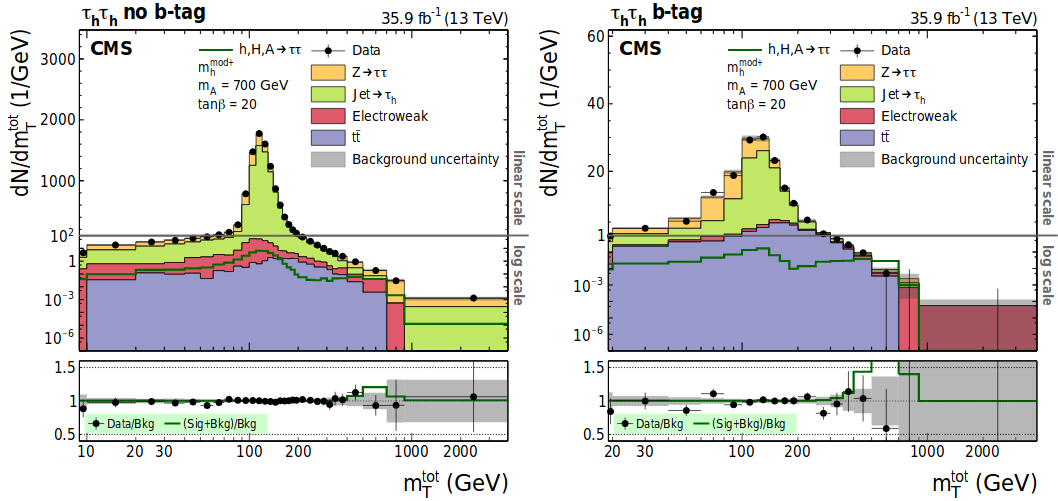
\includegraphics[width=\textwidth]{Images/2016MSSMmttot.png}
%     \caption{Distribution of \mttot in the global no b-tag (left) and b-tag (right) categories.}
%     \label{fig:control_plots}
% \end{figure}

A number of additional steps are needed to determine the \ma -  $\mathrm{tan}\beta$ limits. Signal samples are generated only for the set of \ma mass points to be tested, in the range $90$ to $3200$ GeV. The step size between points increases with \ma to scale with the worsening \mttot resolution. At each \ma -  $\mathrm{tan}\beta$ hypothesis, the masses of the other two Higgs bosons are calculated using results from the Higgs Working Group \cite{Dittmaier:1318996}. In each event category, templates for the h and H are generated by a horizontal morphing \cite{READ1999357} between templates from the two samples
closest in mass. The category acceptance is similarly interpolated from the neighbouring mass
points. All three templates are scaled by the appropriate cross sections and branching ratios and
combined into a single template. The $95\%$ CL upper limit is determined for each point on the \ma -  $\mathrm{tan}\beta$ grid, with the signal strength parameter $\mu$ uniformly scaling the entire signal model. The limit in  $\mathrm{tan}\beta$ is then defined as the point on which this upper limit is found to occur at $\mu = 1.0$. Practically, this is determined by interpolation between the points on either side of this threshold. Note that the SM Higgs boson is added to the background processes. This turns the likelihood ratio into a comparison between the MSSM and the SM Higgs sector hypotheses, and ensures a well defined problem even when the analysis becomes sensitive to the observed Higgs boson at $125\,\mathrm{GeV}$.

The observed and expected limits for the MSSM $m_{\mathrm{h}}^{\mathrm{mod}+}$ and the hMSSM scenarios are given in figure \ref{fig:limits}.

% \begin{figure}
%     \centering
%     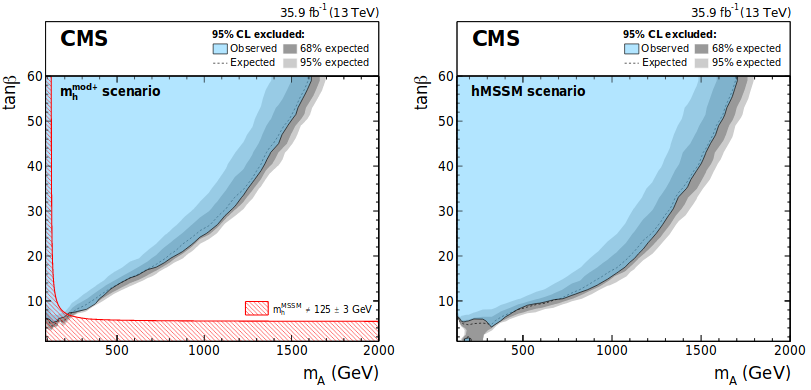
\includegraphics[width=\textwidth]{Images/MSSMlimits.png}
%     \caption{expected and observed $95\%$ CL exclusion contour (left) in the MSSM $m_{\mathrm{h}^{\mathrm{mod}+}}$ and (right) in the hMSSM scenarios. The expected median is shown as a dashed black line. The dark and bright gray bands indicate the 68 and 95 $\%$ confidence intervals for the variation of the expected exclusion. The observed exclusion contour is indicated by the coloured blue area. For the $m_{\mathrm{h}}^{\mathrm{mod}+}$ scenario, those parts of the parameter space, where $m_{\mathrm{h}}$ deviates by more than $\pm 3 \,\mathrm{GeV}$ from the mass of the observed Higgs boson at $125\,\mathrm{GeV}$ are indicated by a red hatched area.}
%     \label{fig:limits}
% \end{figure}

Figure \ref{fig:xslimits} gives model-independent upper limits on the production of a single neutral Higgs boson with mass $m_{\Phi}$. The limits on the cross section times branching fraction, $\sigma\times B(\Phi\rightarrow\tauh\tauh)$, are determined individually for gluon-gluon fusion and b-associated production. In the fit to extract gluon-gluon fusion limits the b-associated contribution is allowed to float freely, and vice versa. This is required as neither the no b-tag or b-tag categories are completely pure in one production mode, and this avoids the need to impose any assumptions about the ratio of cross sections between the two processes.

% \begin{figure}
%     \centering
%     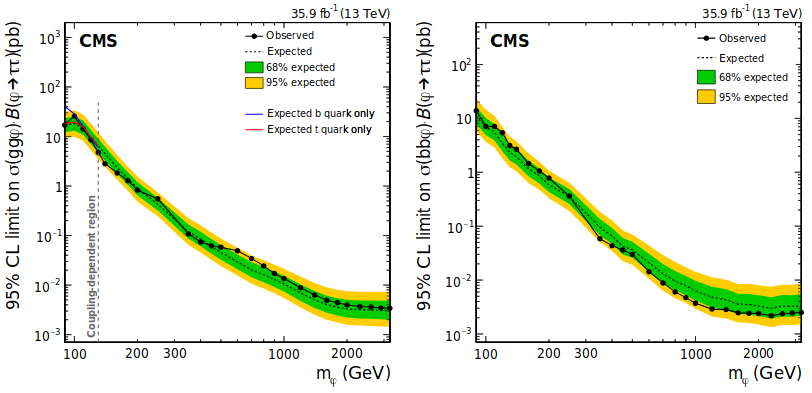
\includegraphics[width=\textwidth]{Images/xslimitsMSSM.png}
%     \caption{Expected and observed $95\%$ CL upper limits for the production of a single narrow resonance, $\Phi$, with a mass between $90\,\mathrm{GeV}$ and $3.2\,\mathrm{TeV}$ in the $\tauh\tauh$ final state (left) for the production via gluon fusion (gg$\Phi$ and (right) in association with b quark (bb$\Phi$). The expected median of the exclusion limit is shown by the dashed line. The dark green and bright yellow bands indicate the 68 and 95$\%$ confidence intervals for the variation of the expected exclusion limit. The black dots correspond to the observed limits.}
%     \label{fig:xslimits}
% \end{figure}


    
% Conclusion
    \chapter{Conclusion}
    This thesis has presented an analysis of proton-proton collision data recorded by the CMS detector during  the 2017 run. The search for a MSSM heavy neutral Higgs boson decaying to tau pairs has been presented. This channel provides a direct probe of the Yukawa couplings between fermions and the Higgs field that give rise to the fermion masses. Results are determined from distributions of the $m_{T}^{\mathrm{tot}}$ variable in the $\tauh\tauh$ final state. Categorisation is used to improve sensitivity to signal and to specific Higgs boson production modes. No significant excess of events above the background expectation is observed. Upper limits at the $95\%$ CL are determined in the $\ma-\mathrm{tan}\,\beta$ parameter space for the $m_{\mathrm{h}}^{\mathrm{max}}$ scenario. Additionally, model-independent limits on the cross section times branching fractions for a single Higgs boson produced via either gluon-gluon fusion or in association with b-quarks are determined for mass hypotheses in the range $90$ to $3200$ GeV.

A new hadronic tau decay identification technique, based on a neural network architecture called recursive neural network. Its performance have been compared to the standard identification technique used in the CMS collaboration. This comparison highlighted a better background rejection in the high signal efficiency region. Some potential improvements to this approach have also been presented.

The LHC has opened a new high-energy frontier in the search for new physics beyond the SM. In 2021 the LHC will re-commence operation to gather even more data, allowing precision measurements as well as search for new physics on a new level. Indeed, new data will offer a much improved sensitivity to signatures of new physics.
    
% Bibliography
    \phantomsection
    \addcontentsline{toc}{chapter}{References}%
    \bibliography{bibliography}
    
    \vspace{2.0cm}
    \textcolor{red}{Refer to \href{http://libguides.lub.lu.se/plagiarism}{LUSEM’s Harvard referencing guidelines} in the Teaching and Learning platform. \url{Lusem.lu.se/asks}}
    % The template provides \hcite and \mcite commands to present hyperlinked references in the 
    % Harvard referencing style '(Author, Year)'  and 'Author (Year)'
    % The template has an automated bibliography section based on references 
    % consistent with entries in the 'bibliography.bib' file 

% % Appendices
%     \appendix
%     \chapter{(Appendix A title)}
%     
\label{appendixA}

This appendix covers mathematical definitions not included in Chapter \ref{sec:TheoryChapter}.

\paragraph{Gama matrices} - $\gamma^{i}$

\begin{table}[h]
    \centering
    \begin{tabular}{c c}
        $\gamma^{0} = \begin{pmatrix} 1 & 0 & 0 & 0 \\ 0 & & 0 & 0 \\ 0 & 0 & -1 & 0 \\ 0 & 0 & 0 & -1 \end{pmatrix}$ & $\gamma^{1} = \begin{pmatrix} 0 & 0 & 0 & 1 \\ 0 & 0 & 1 & 0 \\ 0 & -1 & 0 & 0 \\ -1 & 0 & 0 & 0 \end{pmatrix}$ \\
        $\gamma^{2} = \begin{pmatrix} 0 & 0 & 0 & -i \\ 0 & 0 & i & 0 \\ 0 & i & 0 & 0 \\ -i & 0 & 0 & 0 \end{pmatrix}$ & $\gamma^{3} = \begin{pmatrix} 0 & 0 & 1 & 0 \\ 0 & 0 & 0 & -1 \\ -1 & 0 & 0 & 0 \\ 0 & 1 & 0 & 0 \end{pmatrix}$
    \end{tabular}
\end{table}

\paragraph{Chiral projector} - $\gamma^{5}$

\begin{equation*}
    \gamma^{5} = i \gamma^{0}\gamma^{1}\gamma^{2}\gamma^{3} = \begin{pmatrix} 0 & 0 & 1 & 0 \\ 0 & 0 & 0 & 1 \\ 1 & 0 & 0 & 0 \\ 0 & 1 & 0 & 0 \end{pmatrix}
\end{equation*}

\paragraph{Pauli matrices} - The generators of $SU(2)$ are the $\tau_i$ matrices defined as $\tau_i = \frac{1}{2}\sigma_i$, with $\sigma_i$ as:

\begin{table}[h]
    \centering
    \begin{tabular}{c c c}
        $\sigma_{1} = \begin{pmatrix} 0 & 1 \\ 1 & 0 \end{pmatrix}$ &  $\sigma_{1} = \begin{pmatrix} 0 & -i \\ i & 0 \end{pmatrix}$ & $\sigma_{1} = \begin{pmatrix} 1 & 0 \\ 0 & -1 \end{pmatrix}$
    \end{tabular}
\end{table}

\paragraph{Gell-Mann matrices} - The generators of $SU(3)$ are the $T_i$ matrices defined as $T_i = \frac{1}{2}\lambda_i$, with $\lambda_i$ as:

\begin{table}[h]
    \centering
    \begin{tabular}{c c c}
        $\lambda_1 =  \begin{pmatrix} 0 & 1 & 0 \\ 1 & 0 & 0 \\ 0 & 0 & 0 \end{pmatrix}$ & $\lambda_2 =  \begin{pmatrix} 0 & -i & 0 \\ i & 0 & 0 \\ 0 & 0 & 0 \end{pmatrix}$ & $\lambda_3 =  \begin{pmatrix} 1 & 0 & 0 \\ 0 & -1 & 0 \\ 0 & 0 & 0 \end{pmatrix}$ \\
        $\lambda_4 =  \begin{pmatrix} 0 & 0 & 1 \\ 0 & 0 & 0 \\ 1 & 0 & 0 \end{pmatrix}$ & $\lambda_5 =  \begin{pmatrix} 0 & 0 & -i \\ 0 & 0 & 0 \\ i & 0 & 0 \end{pmatrix}$ & \\
        $\lambda_6 =  \begin{pmatrix} 0 & 0 & 0 \\ 0 & 0 & 1 \\ 0 & 1 & 0 \end{pmatrix}$ & $\lambda_7 =  \begin{pmatrix} 0 & 0 & 0 \\ 0 & 0 & -i \\ 0 & i & 0 \end{pmatrix}$ & $\lambda_8 =  \frac{1}{\sqrt{3}}\begin{pmatrix} 1 & 0 & 0 \\ 0 & 1 & 0 \\ 0 & 0 & -2 \end{pmatrix}$
    \end{tabular}
\end{table}
    
%      \chapter{(Appendix B title)}
%     \input{Sections/Appendix_B}

\end{document}
%----------------------------------------------------------------------------------------------------%
